% arara: pdflatex
% arara: pdflatex
% arara: pdflatex


% options:
% thesis=B bachelor's thesis
% thesis=M master's thesis
% czech thesis in Czech language
% english thesis in English language
% hidelinks remove colour boxes around hyperlinks

\documentclass[thesis=M,english]{FITthesis}[2019/12/23]

\usepackage[utf8]{inputenc} % LaTeX source encoded as UTF-8

% \usepackage{subfig} %subfigures
% \usepackage{amsmath} %advanced maths
% \usepackage{amssymb} %additional math symbols

\usepackage{dirtree} %directory tree visualisation

\usepackage{listings}
\lstset{basicstyle=\ttfamily, language=C++}

\usepackage{amsmath}
\usepackage{tabularx}
\usepackage{xcolor}
\usepackage{minted}
\usepackage{algorithm}
\usepackage{algpseudocode}
\usepackage{float}

\usepackage{siunitx}
\sisetup{round-precision=3,round-mode=figures,scientific-notation=true}

\usepackage{tikz}
\usetikzlibrary{positioning,fit,calc}
\usetikzlibrary{patterns,snakes}

\usepackage{minted}
\usepackage{amsthm,amssymb,amsfonts}
\usepackage{tikz,lipsum,lmodern}
\usepackage[most]{tcolorbox}
\usepackage{multicol}

\usepackage{microtype}
\usepackage{bbm}
\usepackage{regexpatch}
\makeatletter
% Change the `-` delimiter to an active character
\xpatchparametertext\@@@cmidrule{-}{\cA-}{}{}
\xpatchparametertext\@cline{-}{\cA-}{}{}

% % list of acronyms
% \usepackage[acronym,nonumberlist,toc,numberedsection=autolabel]{glossaries}
% \iflanguage{czech}{\renewcommand*{\acronymname}{Seznam pou{\v z}it{\' y}ch zkratek}}{}
% \makeglossaries

% % % % % % % % % % % % % % % % % % % % % % % % % % % % % % 
% EDIT THIS
% % % % % % % % % % % % % % % % % % % % % % % % % % % % % % 

\department{Department of Theoretical Computer Science}
\title{Distributed Sparse Matrix-Vector Multiplication}
\authorGN{Boris} %author's given name/names
\authorFN{Rúra} %author's surname
\author{Boris Rúra} %author's name without academic degrees
\authorWithDegrees{Bc. Boris Rúra} %author's name with academic degrees
\supervisor{doc. Ing. Ivan Šimeček, Ph.D.}
\acknowledgements{The access to the computational infrastructure of the OP VVV funded project CZ.02.1.01/0.0/0.0/16\_019/0000765 ``Research Center for Informatics'' is also gratefully acknowledged.}
\abstractEN{The aim of this thesis is to research possibilities of distributing sparse matrix-vector multiplication among multiple processes using MPI and CSR5 storage format.
The result of this research is a C++ library \texttt{dim}, which provides the building blocks for distributed 
SpMV using CSR5.
The potential speedup of distributed SpMV is then benchmarked on a conjugate gradient algorithm implementation against 
a single-process CSR5 based implementation as well as PETSc based multi-process implementation.}
\abstractCS{Cílem práce bylo prozkoumat možnosti distribuovaného násobení řídké matice vektorem několika
procesy s použitím MPI a CSR5. Výsledkem tohto výzkumu je C++ knihovna \texttt{dim}, která poskytuje potřebné 
stavební bloky pro distribuované násobení řídkých matic vektorem za pomoci formátu CSR5. Potencionálni zrychlení 
distribuovaného násobení řídké matice vektorem pak bylo meřeno na implementaci metody konjugovaných gradientů
a porovnávano s jednoprocesovou implementací založenou na CSR5 i distribuovanou implementací pomocí PETSc.}
\placeForDeclarationOfAuthenticity{Prague}
\keywordsCS{násobení řídké matice vektorem, C++, OpenMP, MPI, metoda konjugovaných gradientů, CSR5, HDF5}
\keywordsEN{sparse matrix-vector multiplication, C++, OpenMP, MPI, conjugate gradient method, CSR5, HDF5}
\declarationOfAuthenticityOption{1} %select as appropriate, according to the desired license (integer 1-6)
% \website{http://site.example/thesis} %optional thesis URL



\newtcolorbox{boxyyy}[2][]{sidebyside,
    lower separated=false,
    righthand ratio=0.56, % to define right-hand fraction
    colback=white,
    colframe=white!20!gray,fonttitle=\bfseries,
    colbacktitle=white!10!gray,enhanced,
    attach boxed title to top left={xshift=1cm,
            yshift=-2mm},
    title=#2,#1}

\newcommand*{\captionsource}[2]{%
    \caption[{#1}]{%
        #1%
        \\\hspace{\linewidth}%
        \textbf{Source:} #2%
    }%
}
\newcommand{\csre}[1]{\mintinline{C++}!#1!}
\newcommand{\pluseq}{\mathrel{+}=}

\algnewcommand{\algorithmicand}{\textbf{ and }}
\algnewcommand{\algorithmicor}{\textbf{ or }}
\algnewcommand{\OR}{\algorithmicor}
\algnewcommand{\AND}{\algorithmicand}
\algnewcommand{\var}{\texttt}


\begin{document}

\tableofcontents
% \newacronym{CVUT}{{\v C}VUT}{{\v C}esk{\' e} vysok{\' e} u{\v c}en{\' i} technick{\' e} v Praze}
% \newacronym{FIT}{FIT}{Fakulta informa{\v c}n{\' i}ch technologi{\' i}}

\setsecnumdepth{part}
\chapter{Introduction}

Sparse matrix-vector multiplication is a fundamental computational kernel used for many
scientific computations, such as graph algorithms, numerical analysis, conjugate gradients
as well as some machine learning algorithms, such as support vector machine.
While matrix-vector multiplication is a simple multiplication task, it is non-trivial to load balance
properly for every sparsity structure matrix when parallelized.

The conjugate gradient algorithm is one of the best known iterative methods which can be used, to solve large
symmetric positive definite linear systems. With sparse matrix-vector multiplication being the most
computationally intensive step of a conjugate gradient iteration, parallelizing the kernel and distributing
the computation across multiple nodes can result in significantly shorter iteration times.

The goals of this thesis are to:

\begin{enumerate}
    \item Review existing sparse matrix storage formats.
    \item Review existing approaches to parallel SpMV\@.
    \item Implement the parallel SpMV algorithm introduced in~\cite{liu2015csr5}.
    \item Introduce efficient on-disk storage format for sparse-matrix format outlined
          in~\cite{liu2015csr5} suitable for distributed version.
    \item Implement a distributed version of parallel SpMV (D-CSR5) using the parallel implementation
          and storage format introduced in this thesis.
    \item Measure and review the viability of distributing SpMV\@.
    \item Benchmark the distributed implementation against PETSc suite.
\end{enumerate}



\setsecnumdepth{all}




\chapter{Overview of used technologies}\label{tech}

% TODO
This chapter introduces the technologies used in the implementation of this thesis.
SIMD parallel processing, as well as SSE/AVX instructions sets, are defined in Section~\ref{tech:simd}.
Section~\ref{tech:omp} introduces OpenMP API, used to parallelize the computation.
Section~\ref{tech:mpi} introduces MPI, a Message Passing
Interface, used for inter-process communication in the distributed SpMV implementation.  Lastly
Section~\ref{theory:MMEF} introduces Matrix Marked Exchange Format for storing sparse and dense matrices,
and Section~\ref{theory: HDF5} introduces Hierarchical Data Format v5, used for efficient sparse matrix
on-disk storage as described in Section~\ref{csr5:onDisk}.


\section{SIMD}\label{tech:simd}

As defined in Flynn's taxonomy, Single Instruction Multiple Data (or SIMD) is a type of parallel
processing, where a single instruction is applied to multiple data streams.

\begin{figure}[htp]
    \centering
    \begin{tikzpicture}
        % tiles

        \coordinate (xmm0) at (0, 0);

        \draw[step=0.5cm,gray,very thin] ($ (xmm0) + (0, 0) $) grid ($ (xmm0) + (2, 0.5)$);
        \foreach \i in {0,...,3}
        \node (xmm0\i) at ($(xmm0) + (\i * 0.5 + 0.25, 0.25)$) {$\i$};

        \node at ($(xmm0) + (-1, 0.25)$) {\csre{xmm0}};

        \coordinate (xmm1) at (0, -1);

        \draw[step=0.5cm,gray,very thin] ($ (xmm1) + (-0.01, 0) $) grid ($ (xmm1) + (2, 0.5)$);
        \foreach \i [evaluate=\i as \ff using int(3-\i)] in {0,...,3}
        \node (xmm1\i) at ($(xmm1) + ({\i * 0.5 + 0.25}, 0.25)$) {$\ff$};

        \node at ($(xmm1) + (-1, 0.25)$) {\csre{xmm1}};


        \foreach \i in {0,...,3}
            {
                \draw [-stealth] (xmm0\i) -- (xmm1\i);
                \node [circle, fill=white!100, draw=black!50, scale=0.35] at ($(xmm0\i) + (0, -0.45)$) {+};
            }

        \coordinate (xmm3) at (0, -2);

        \draw[step=0.5cm,gray,very thin] ($ (xmm3) + (-0.01, 0) $) grid ($ (xmm3) + (2, 0.5)$);
        \foreach \i in {0,...,3}
        \node (xmm2\i) at ($(xmm3) + ({\i*0.5 + 0.25}, 0.25)$) {$3$};

        \node at ($(xmm3) + (-1, 0.25)$) {\csre{xmm2}};

        \foreach \i in {0,...,3}
            {
                \draw [-stealth] (xmm1\i) -- (xmm2\i);
            }


        \draw [dotted] (-1, -1.3) -- (6, -1.3);
        \node (st) [anchor=east, scale=0.8] at (6, -1.1) {\csre{vpaddd xmm2, xmm2, xmm1}};

        \foreach \i in {0,...,4}
        \draw [dotted, draw=red!90, line width = 0.3mm] (\i*0.5, 0.5) -- (\i*0.5, -2);

        \foreach \i in {0,...,3}
        \node [above=0.5mm of xmm0\i, anchor=south] {$L_{\i}$};

    \end{tikzpicture}
    \caption{Example of SIMD addition using SSE}\label{tech:simd:fig}
\end{figure}

Modern CPUs provide Streaming SIMD Extensions (or SSE) Instruction Set Extensions which work on 16 byte
registers, as well as Advanced Vector Extensions (or AVX), which work with 32-byte registers.
To illustrate, Figure~\ref{tech:simd:fig} shows addition (single instruction) of two
four-integer arrays (multiple data) using the \csre{vpaddd} instruction from SSE\@. The data streams
are sometimes referred to as lanes (marked as \(L_0\)-\(L_3\) in Figure~\ref{tech:simd:fig}).

In C++, there are several ways to achieve vectorization\footnote{Note that the target architecture needs
    to be specified for the compiler to enable vector instructions.}.
First of these are SIMD intrinsics. Intrinsics
are assembly-coded functions that let you use C++ function calls and variables in place of assembly
instructions, improving readability. To generate the \csre{vpaddd} instruction from Figure~\ref{tech:simd:fig}
intrinsic \csre{_mm_add_epi32} can be used.

Vectorization may also be achieved by using a pragma directive from OpenMP described in Section~\ref{tech:omp},
as shown in Figure~\ref{tech:simd:omp}.

\begin{figure}[htp]
    \centering
    \begin{minted}{C++}
        #pragma omp simd
        for (int lane = 0; lane < 4; ++lane)
            c[i] = a[i] + b[i]
    \end{minted}
    \caption{Vectorization using OpenMP}\label{tech:simd:omp}
\end{figure}

Lastly, standard C++ may be used to produce vectorized code by utilizing \csre{<execution>} header
and its \csre{par_unseq} and \csre{unseq} execution policies. These however only aid the compiler
auto-vectorization and do not guarantee the vector instructions will actually be used.


\section{OpenMP}\label{tech:omp}

OpenMP API is defined by a collection of compiler directives, library routines, and environment variables.
It provides a model for parallel programming that is portable across architectures
from different vendors. Compilers from numerous vendors support the OpenMP API\cite{openmp18}.
OpenMP uses the fork-join model of parallel execution.

For C++ the directives have the form of preprocessor \texttt{\#pragma} directives, with the following
syntax.
\begin{minted}{c++}
    #pragma omp <directive-name> [clause[[,]clause]...] new-line
\end{minted}

To enable OpenMP, the compiler must be invoked with the \csre{-fopenmp}
switch for GCC/clang-based compilers, while MSVC accepts the \csre{/openmp} flag.

\subsection{\texttt{parallel} directive}

\texttt{parallel} directive marks a region to be executed in parallel. A \textbf{team} within the parallel
region is a set of one or more threads participating in the execution of this region. If the team has at
least two active threads, the parallel region is \textbf{active}, else it is called \textbf{inactive}.

The threads in OpenMP have a \textbf{numerical identifier}. In this thesis, this numerical identifier will be
referred to as \textbf{thread id}\footnote{Not the thread id in the context of an OS.}.
The thread which has thread id equal to 0 is called the \textbf{master}
thread within the team while other consecutive thread ids are assigned to remaining threads.
It can be obtained by calling \mintinline{C++}{omp_get_thread_num}.

\subsection{\texttt{for} directive}

Referred to as Worksharing-Loop Construct in~\cite{openmp18}. It specifies that the iterations
of the associated loop(s) will be executed in parallel by the threads of the currently active
team. As a result, the execution is only parallelized if the loop is performed inside of a
\texttt{parallel} region in the first place.

All of the allowed clauses for the directive can be found in~\cite{openmp18}, the only relevant one
for this thesis is \texttt{schedule}, specified as \\
\texttt{schedule([modifier [, modifier]:]kind[, chunk\_size])}. Modifier isn't immediately relevant
but \texttt{kind} is. \textbf{kind} specifies, how the work is distributed among the threads.

When \texttt{dynamic} kind is specified, the iterations are distributed among threads dynamically.
Meaning when a thread finishes processing its assigned chunk (of \texttt{chunk\_size} elements),
it requests a new chunk until no chunks remain.

\texttt{static} kind distributes chunks of \texttt{chunk\_size} among the participating threads in a
round-robin fashion. This kind is used heavily in the computational kernel described in Section~\ref{csr5:spmv}.

\texttt{parallel} and \texttt{for} directives may be combined as shown in Figure~\ref{tech:omp:loop},
to create a so-called parallel worksharing-loop construct. Which is a shortcut for specifying
\texttt{parallel} construct containing a worksharing-loop.

\begin{figure}[htp]
    \begin{minted}{C++}
    #pragma omp parallel for
    for (int i = 0; i < num_iters; ++i)
        // performed in parallel
    \end{minted}
    \caption{Loop parallelized using OpenMP directives.}\label{tech:omp:loop}
\end{figure}


OpenMP contains many other primitives for parallel programming such as atomics, barriers
and semaphores and can also be used to vectorize loops using the \texttt{simd} construct as shown
in Figure~\ref{tech:simd:omp}.

\section{MPI}\label{tech:mpi}

MPI (Message-Passing Interface) is a message-passing library interface specification.
All parts of this definition are significant. MPI addresses primarily the message-passing parallel
programming model, in which data is moved from the address space of one process to
that of another process through cooperative operations on each process.

Extensions to the
“classical” message-passing model are provided in collective operations, remote-memory
access operations, dynamic process creation, and parallel I/O, which is used to speed-up loading
sparse matrices from disk as described in Section~\ref{dspmv:load}. MPI is a specification, not
an implementation; there are multiple implementations of MPI. This specification is for a
library interface; MPI is not a language, and all MPI operations are expressed as functions,
subroutines, or methods, according to the appropriate language bindings which, for C and
Fortran, are part of the MPI standard.
\cite{mpi40}

\subsection{Initialization}\label{tech:mpi:init}

Before invoking any MPI routines, a participating process must call \csre{MPI_Init} which
initializes internal state of an MPI implementation, which must then be freed by calling
\csre{MPI_Finalize}.

\subsection{Communicators}\label{tech:mpi:comm}

Most MPI routines require a communicator. In MPI a \textbf{communicator} a communicator is a
context for a communication operation~\cite{mpi40}. Participating processes are also referred to as
\textbf{process group} and are each process is assigned a non-negative \textbf{rank} within this group.

\begin{figure}[htp]
    \centering
    \begin{tikzpicture}
        \node (p0) [circle, draw=red!90] at (0, 0) {0};
        \node (p1) [right=of p0, circle, draw=green!90]{1};
        \node (p2) [right=of p1, circle, draw=blue!90]{2};
        \node (p3) [right=of p2, circle, draw=orange!90]{3};

        \node (commWorld) [draw=black!90, fit={(p0) (p1) (p2) (p3)}, rounded corners] {};
        \node [above=0.1cm of commWorld, anchor=south] {\csre{MPI_COMM_WORLD}};

        \node (p11) [below=1.5cm of p1, circle, draw=green!90]{0};
        \node (p21) [right=of p11, circle, draw=orange!90]{1};

        \node (commNew) [draw=black!90, fit={(p11) (p21)}, rounded corners] {};

        \draw [-stealth] (commWorld) -- (commNew);

        \node (mpiSpl) [fill=white!100, draw=gray!90] at ($(commWorld)!0.5!(commNew)$) {\csre{MPI_Comm_split}};

    \end{tikzpicture}
    \caption{Splitting a communicator to create a new one}\label{tech:mpi:comm:fig}
\end{figure}

MPI implementations provide some predefined
communicators such as \csre{MPI_COMM_WORLD} which contains every process accessible
after initialization described in Section~\ref{tech:mpi:init} and \csre{MPI_COMM_SELF}
which contains only the calling process (self). One of the most common methods for creating
new communicators is splitting an existing one. This can be done by calling
\csre{MPI_Comm_split} (Shown in Figure~\ref{tech:mpi:comm:fig}) and is utilized for synchronization
of sub-results as explained in Section~\ref{dspmv:sync}.

\subsection{MPI operations}\label{tech:mpi:op}

An MPI operation is a sequence of steps performed to establish and enable data transfer/synchronization\cite{mpi40}.
It consists of four stages:

\begin{itemize}
    \item \textbf{Initialization} hands over the argument list to the operation, but not the content
          of the data buffers.
    \item \textbf{Starting} hands over the control of the data buffers.
    \item \textbf{Completion} returns control of the content of the data buffers and indicates
          that output buffers and arguments may have been updated.
    \item \textbf{Freeing} returns the control of the rest of the argument list to the caller.

\end{itemize}


\subsection{\texttt{MPI\_Allgatherv}}\label{tech:mpi:gat}

\csre{MPI_Allgatherv} is a collective, blocking operation, which is useful for distributing arrays of
data between processes. A \textbf{collective} operation in MPI is an operation in which a group of
processes participates, for which the completion
stage may or may not finish before all processes in the group have started the operation.
A \textbf{blocking} operation combines all four stages outlined in Section~\ref{tech:mpi:op}.

\begin{figure}[htp]
    \centering
    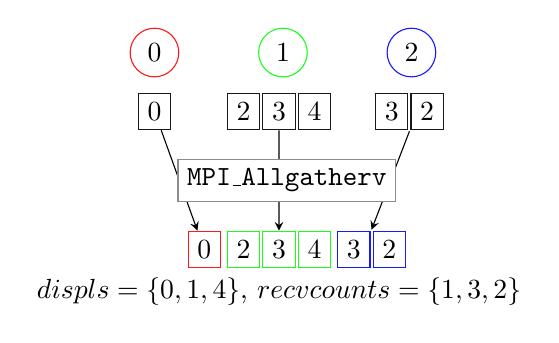
\begin{tikzpicture}
        \node (p0) [circle, draw=red!90] at (0, 0) {0};
        \node (p1) [right=of p0, circle, draw=green!90]{1};
        \node (p2) [right=of p1, circle, draw=blue!90]{2};

        \coordinate (p0data) at ($(p0) + (0, -0.75)$);
        \coordinate (p1data) at ($(p1) + (-0.5, -0.75)$);
        \coordinate (p2data) at ($(p2) + (-0.25, -0.75)$);
        \coordinate (result) at ($(p1) + (0, -2.5)$);

        \node (p00) [rectangle, draw=black!90] at (p0data) {0};
        \node (p0r) [rectangle, draw=red!90] at ($(result) + (-1, 0)$) {0};

        \foreach \x [evaluate=\x as \ff using int(\x+2)] in {0,...,2}
            {
                \node (p1\x) [rectangle, draw=black!90] at ($(p1data) + (\x * 0.45, 0)$) {\ff};
                \node (p1r\x) [rectangle, draw=green!90] at ($(result) + (\x * 0.45 - 0.5, 0)$) {\ff};
            }

        \foreach \x [evaluate=\x as \ff using int(3-\x)] in {0,...,1}
            {
                \node (p2\x) [rectangle, draw=black!90] at ($(p2data) + (\x * 0.45, 0)$) {\ff};
                \node (p2r\x) [rectangle, draw=blue!90] at ($(result) + (\x * 0.45 + 0.9, 0)$) {\ff};
            }

        \draw [-stealth] (p00) -- (p0r);
        \draw [-stealth] (p11) -- (p1r1);
        \draw [-stealth] ($(p20)!0.5!(p21) + (0, -0.25)$) -- ($(p2r0)!0.5!(p2r1) + (0, 0.25)$);


        \node (mpiRed) [fill=white!100, draw=gray!90] at ($(p11)!0.5!(p1r1) + (0.1, 0)$) {\texttt{MPI\_Allgatherv}};

        \node [below=3mm of p1r1, anchor=center] {$\var{displs} = \{0, 1, 4\}\text{, }\var{recvcounts} = \{1, 3, 2\}$};


    \end{tikzpicture}
    \caption{Distributing data with \texttt{MPI\_Allgatherv}}\label{tech:mpi:allgat:fig}
\end{figure}

The routine takes an input array, its size, an output array, \texttt{displs} and \texttt{recvcounts}.
The last two arrays contain offset into the output array and the amount of contributed data for each
participating process respectively and have to be the same for every participating process.

\subsection{\texttt{MPI\_Allreduce}}\label{tech:mpi:red}

\csre{MPI_Allreduce} performs parallel reduction among all participating processes. Different reduction
operators can be used, such as \csre{MPI_SUM}, \csre{MPI_PROD}, \csre{MPI_MAX} etc. The implementation
produced alongside this thesis mostly uses its non-blocking counterpart, \csre{MPI_Iallreduce}.
A \textbf{non-blocking} operation
combines the first two MPI operation stages into a single non-blocking call. It then must be finished by
either waiting by calling \csre{MPI_Wait} (or \csre{MPI_Waitall} if waiting on multiple operations).
This operation is the backbone of synchronization for parallel SpMV outlined in Section~\ref{dspmv:sync}.

\begin{figure}[htp]
    \centering
    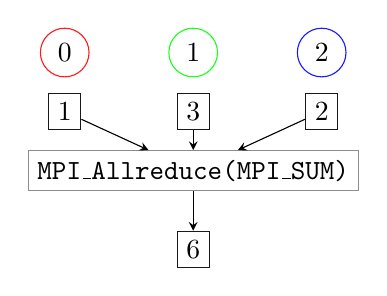
\begin{tikzpicture}
        \node (p0) [circle, draw=red!90] at (0, 0) {0};
        \node (p1) [right=of p0, circle, draw=green!90]{1};
        \node (p2) [right=of p1, circle, draw=blue!90]{2};

        \node (p00) [rectangle, draw=black!90] at ($(p0) + (0, -0.75)$) {1};
        \node (p10) [rectangle, draw=black!90] at ($(p1) + (0, -0.75)$) {3};
        \node (p20) [rectangle, draw=black!90] at ($(p2) + (0, -0.75)$) {2};

        \node (red) [fill=white!100, draw=gray!90] at ($(p1) + (0, -1.5)$) {\texttt{MPI\_Allreduce(MPI\_SUM)}};

        \foreach \x in {0,...,2}
        \draw [-stealth] (p\x0) -- (red);

        \node (result) [rectangle, draw=black!90] at ($(p1) + (0, -2.5)$) {6};

        \draw[-stealth] (red) -- (result);
    \end{tikzpicture}
    \caption{Performing parallel reduction with \texttt{MPI\_Allreduce}}\label{tech:mpi:allred:fig}
\end{figure}

\section{PETSc}\label{tech:petsc}

Portable, Extensible Toolkit for Scientific computation (PETSc) is a suite of data structures and routines
for scalable solutions of scientific applications modeled by partial differential equations.
It supports MPI, and GPUs through CUDA, HIP or OpenCL, as well as hybrid MPI-GPU parallelism~\cite{petsc-web-page}.

PETSc contains three main algebraic objects \csre{Mat} for matrices, \csre{Vec} for vectors and \csre{IS}
for index sets indexing into the previous two. While it also contains many other components, only \csre{Mat}
and \csre{Vec} are immediately relevant to this thesis.


\section{Matrix Market Exchange Format}\label{theory:MMEF}

Matrix Market Exchange Format is a textual format, used as a native format in Matrix Market\footnote{
    Matrix Market is a repository of sparse matrices which can be found at https://math.nist.gov/MatrixMarket/
}.
It has two flavors, Array format for dense matrices, Coordinate format for sparse matrices~\cite{mmef}.

% TODO: citations

\subsection{General Format Specification}

All Matrix Market exchange format files contain three sections, which must appear in order:

\begin{enumerate}
    \item \textbf{Header} First line of a file, must follow the template:
          \begin{lstlisting}
    %%MatrixMarket object format [qualifier...]
\end{lstlisting}
          Where object type indicates the mathematical object (e.g., vector or matrix)
          stored in the file. Type indicates the format (array or coordinate) used to store
          the object. Qualifiers are used to indicate special properties of the stored
          object (e.g., symmetry, field). Their number, as well as allowed values, depends on
          the stored object.
    \item \textbf{Comments} Zero or more line of comments\footnote{Comments are lines starting with \%.}.
    \item \textbf{Data} Remainder of the file contains data representing the object.
          The format of data is dependent on the stored object, but for simplicity,
          each data entry should occupy a single line.
\end{enumerate}

\subsection{Coordinate Format for Sparse Matrices}

Header format for sparse matrices:
\begin{lstlisting}
%%MatrixMarket matrix coordinate <field> <symmetry>
\end{lstlisting}

Where:
\begin{itemize}
    \item \textbf{field} determines the type and number of values listed for each entry
          and is one of: Real, Complex, Integer or Pattern.
    \item \textbf{symmetry} determines how to interpret matrix entries
          and is one of: General, Symmetric, Skew-Symmetric or Hermitian.
\end{itemize}

While data is specified as:
\begin{lstlisting}
    M N L
    I J A(I, J)
    I J A(I, J)
    ...
\end{lstlisting}

First line of data contains exactly three integers:
\begin{itemize}
    \item \csre{M} - number of rows.
    \item \csre{N} - number of columns.
    \item \csre{L} - number of non-zero entries that follows.
\end{itemize}

The following \csre{L} lines each contain \csre{I} - the row index, \csre{J} - the column index
and the corresponding value. Indices are 1-based. Entries not explicitly provided are considered
to be zero, except for those known by symmetry.


\section{HDF5}\label{theory:HDF5}

HDF5 is a data model, library, and file format for storing and managing data.
It supports an unlimited variety of data types and is designed for flexible and
efficient I/O for high volume and complex data. HDF5 is portable and is extensible,
allowing applications to evolve in their use of HDF5. The HDF5 Technology suite includes
tools and applications for managing, manipulating, viewing, and analyzing data in the HDF5 format.
\cite{hdf5} HDF5 is defined by HDF5 File Format Specification, which specifies the bit-level
organization of an HDF5.

\subsection{HDF5 Abstract Data Model}

The HDF5 data model defines building blocks for data organization and specification in HDF5.
It's two primary objects are \textbf{groups} and \textbf{datasets}.

\subsubsection{Group}

HDF5 groups organize data. Every file contains at least a root group.
Each group can contain other groups or be linked to objects in other files.

\begin{figure}[!h]
    \centering
    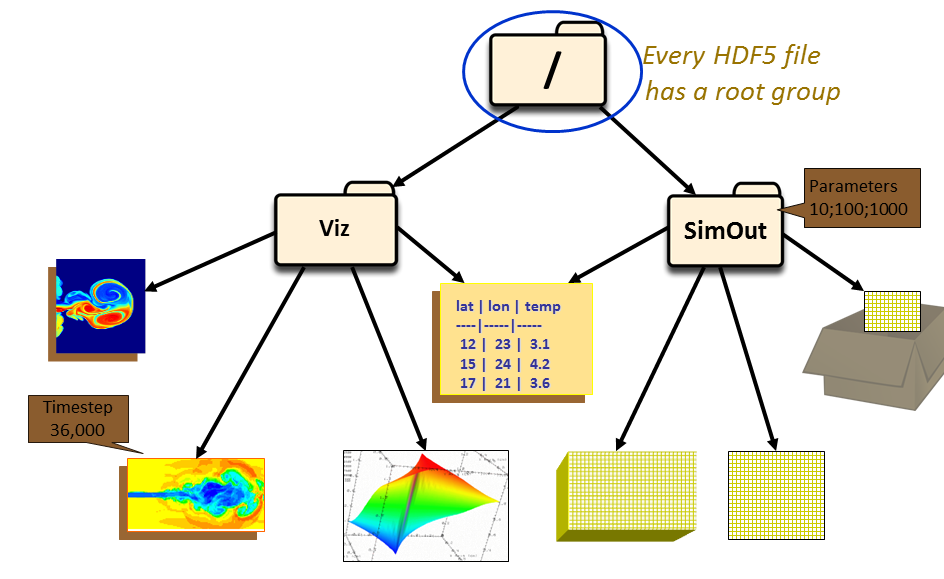
\includegraphics[scale=0.3]{static/group.png}
    \caption{HDF5 Group (Source:~\cite{hdf5})}
\end{figure}

Working with groups and their members is similar to working with files and directories in UNIX.
Objects are described by giving their pathnames (e.g., \texttt{/Viz}).

\subsubsection{Dataset}

Datasets organize and contain the "raw" data. They consist of raw data and metadata needed to describe it.
The metadata needed to describe a dataset consists of datatypes, dataspaces, properties and optionally
attributes.

\begin{figure}[H]
    \centering
    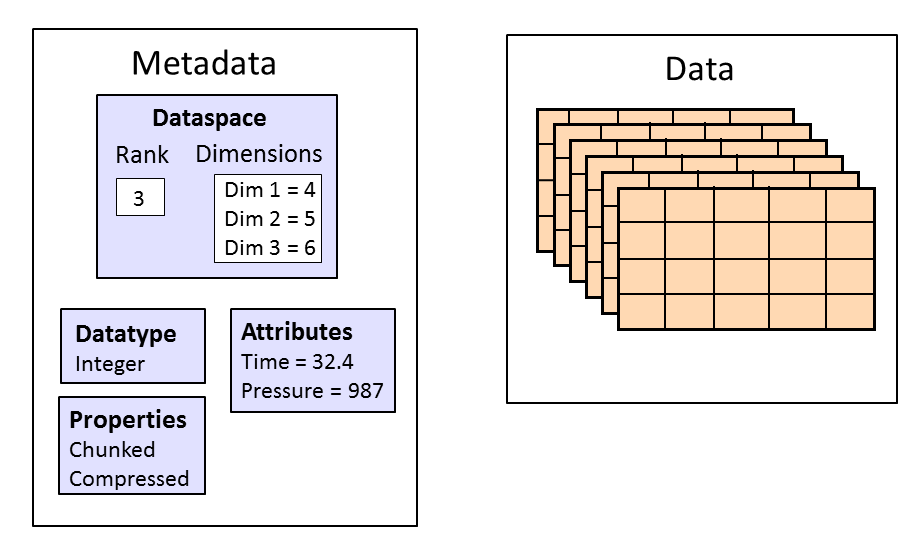
\includegraphics[scale=0.3]{static/dataset.png}
    \caption{HDF5 Dataset (Source:~\cite{hdf5})}
\end{figure}

\subsubsection{Datatype}

Datatypes describe individual elements in dataset. There are two groups of datatypes:
\begin{itemize}
    \item \textbf{pre-defined} - created by HDF5, contain standard datatypes that are stable across platforms
          (e.g IEEE-754 encoded floating point), as well as native datatypes (e.g. \texttt{double} on platform
          on which the application is running).
    \item \textbf{derived} - created or derived from pre-defined datatypes (e.g. a string).
\end{itemize}

\subsubsection{Dataspace}

Dataspaces describe the layout of datasets elements. It may be empty (NULL), contain a single element (scalar),
or an array\footnote{The number of dimensions of the array is referred to as rank of the dataspace.}. They provide
a logical layout of the dataset stored in a file (including rank and dimensions). As well as the application's data buffers
and data elements participating in I/O. Thus an application can select subsets of a dataset.
% TODO: reference the chapter which will discuss hyperslabs more in depth.

\begin{figure}[H]
    \centering
    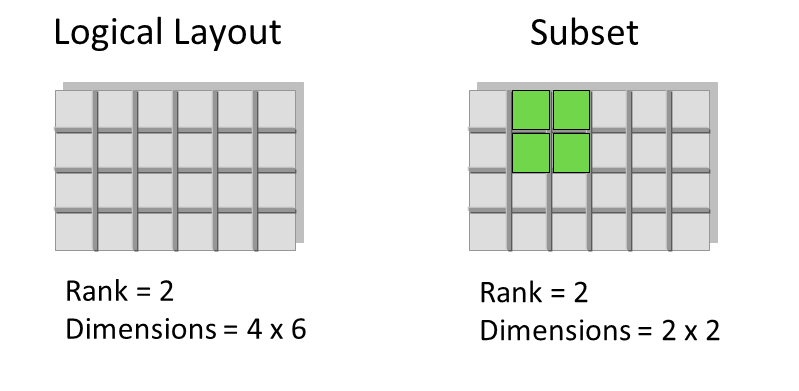
\includegraphics[scale=0.3]{static/dataspace.png}
    \caption{HDF5 Dataspace (Source:~\cite{hdf5})}
\end{figure}



\subsubsection{Attribute}

Attributes may optionally be associated with objects. An attribute consists of a name-value pair.
They are similar to datasets in that they too have a datatype and dataspace. However, they do not
support partial I/O and cannot be compressed or extended.


\chapter{Sparse matrix storage formats}

Section~\ref{smsf:spm} of this chapter introduces sparse matrices. Sections~\ref{smsf:coo} and~\ref{smsf:csr}
provide a quick overview of the two most used storage formats for sparse matrices in Coordinate format (COO)
and Compressed Sparse Row (CSR). Compressed Sparse Row 5 introduced in \cite{liu2015csr5} is then outlined
in Section~\ref{csr5Intro}.


\section{Sparse matrices}\label{smsf:spm}

A matrix is a rectangular array of numbers. The numbers in the array
are called the entries in the matrix~\cite{anton14}. Matrix entries are usually addressed
by the column and row in the rectangle they occupy.

In numerical analysis and scientific computing, a sparse matrix or sparse array
is a matrix in which most of the elements are zero. There is no strict definition
regarding the proportion of zero-value elements for a matrix to qualify as sparse,
but a common criterion is that the number of non-zero elements is roughly equal
to the number of rows or columns. By contrast, if most elements are non-zero,
the matrix is considered dense.
The number of zero-valued elements divided by the total number of elements (e.g., m × n for an m × n matrix) is sometimes referred to as the sparsity of the matrix.
\cite{efficientSDMM} The number of non-zero elements of a sparse matrix is usually denoted
as \(n_{nz}\) number of columns as \(n\) and the number of rows as \(m\).

To better illustrate the storage formats, let us define sparse matrix \(A\).
\begin{equation*}
    A =
    \begin{pmatrix}
        1 & 0 & 2 & 0 \\
        0 & 3 & 0 & 0 \\
        4 & 0 & 5 & 0 \\
        6 & 0 & 0 & 7
    \end{pmatrix}
\end{equation*}

\section{Coordinate (COO)}\label{smsf:coo}

Coordinate storage format, commonly referred to as COO, is the simplest of the three formats presented in this
chapter. COO stores the matrix in a structure consisting of three arrays of length $n_{nz}$\cite{saad03:IMS}:

\begin{enumerate}
    \itemsep=0em
    \item[vals] an array containing all the real (or complex) values of the nonzero elements of A in any order.
    \item[row\_idx] an integer array containing their row indices.
    \item[col\_idx] a second integer array containing their column indices.
\end{enumerate}

\begin{table}[h!]
    \centering
    \begin{tabular}{ |l||c|c|c|c|c|c|c| }
        \hline
        vals     & 1 & 2 & 3 & 4 & 5 & 6 & 7 \\
        \hline
        row\_idx & 0 & 0 & 1 & 2 & 2 & 3 & 3 \\
        \hline
        col\_idx & 0 & 2 & 1 & 0 & 2 & 0 & 3 \\
        \hline
    \end{tabular}
    \caption{$A$ stored in COO format}
\end{table}

As shown in Algorithm~\ref{coo:spmv}, to perform SpMV with a matrix stored in the COO format, it is necessary
to iterate over all non-zero elements, extracting their value, column index, and row index from the
relevant arrays in the COO structure. Then performing the multiplication \(\var{value} \cdot \var{x[col]}\) and
finally add the sub-result to \(\var{y[row]}\). This algorithm is not well suited for parallelization,
as all the additions to the result vector \(\var{y}\) would have to be atomic operations. It may also
degrade single-thread performance as the order of non-zero elements is not specified, meaning accesses to $\var{x}$
as well as $\var{y}$ are random and thus may not have the best cache locality.

\begin{algorithm}
    \caption{SpMV for matrix stored in COO format}\label{coo:spmv}
    \begin{algorithmic}
        \Function{spmv}{$\var{A}$, $\var{x}$}
        \State $\var{y} \gets \text{result vector}$

        \For{\var{i = 0; i < nnz; ++i}}
        \State $\var{value} \gets \var{A.vals}$
        \State $\var{col} \gets \var{A.col\_idx[i]}$
        \State $\var{row} \gets \var{A.row\_idx[i]}$
        \State $\var{y[row]} \pluseq \var{value} \cdot \var{x[col]}$
        \EndFor

        \Return $\var{y}$
        \EndFunction
    \end{algorithmic}
\end{algorithm}

\section{Compressed Sparse Row (CSR)}\label{smsf:csr}

Compressed Sparse Row is probably the most popular format for storing general sparse matrices.
\cite{saad03:IMS} Similarly to the coordinate format, it too consists of three arrays.

% TODO: better lstinline.
\begin{enumerate}
    \itemsep=0em
    \item[vals] a real array of size $n_{nz}$ containing all the real (or complex) values of the nonzero elements of $A$
        stored in row major order.
    \item[col\_idx] a second integer array of size $n_{nz}$ containing their column indices.
    \item[row\_ptr] an integer array of size $m + 1$ containing offsets into \lstinline{vals} and
        \lstinline!col_idx!, at which each row of the matrix begins.
\end{enumerate}

Storing only $m + 1$ elements in \csre{row_ptr} array, leads to non-negligible storage savings.

\begin{table}[h!]
    \centering
    \begin{tabular}{ |l||c|c|c|c|c|c|c| }
        \hline
        vals     & 1 & 2 & 3 & 4 & 5 & 6 & 7 \\
        \hline
        col\_idx & 0 & 2 & 1 & 0 & 2 & 0 & 3 \\
        \hline
    \end{tabular} \\
    \begin{tabular}{ |l||c|c|c|c|c| }
        \hline
        row\_ptr & 0 & 2 & 3 & 5 & 6 \\
        \hline
    \end{tabular}
    \caption{$A$ stored in CSR format}
\end{table}

SpMV with matrix in CSR format lends itself to parallelization better than the COO format. Since
CSR groups the non-zero elements by their rows, the outer loop of Algorithm~\ref{csr:spmv}
can be parallelized with no synchronization necessary (no overlapping outputs in \(\var{y}\)).
The issue with the parallelized version of this algorithm is load-balancing, as some rows may have
disproportionately more non-zero elements than others.

\begin{algorithm}
    \caption{SpMV for matrix stored in CSR format}\label{csr:spmv}
    \begin{algorithmic}
        \Function{spmv}{$\var{A}$, $\var{x}$}
        \State $\var{y} \gets \text{result vector}$
        \For{\var{row = 0; row < m; ++row}}
        \State $\var{start} \gets \var{A.row\_ptr[row]}$
        \State $\var{stop} \gets \var{A.row\_ptr[row + 1]}$
        \State $\var{row\_result} \gets 0$
        \For{\var{i = start; i < stop; ++i}}
        \State $\var{col} \gets \var{A.col\_idx[i]}$
        \State $\var{value} \gets \var{A.vals[i]}$
        \State $\var{row\_result} \pluseq \var{value} \cdot \var{x[col]}$
        \EndFor
        \State $\var{y[row]} \gets \var{row\_result}$
        \EndFor
        \Return $\var{y}$
        \EndFunction
    \end{algorithmic}
\end{algorithm}

\section{Compressed Sparse Row 5 (CSR5)}\label{csr5Intro}

To achieve near-optimal load balance for matrices with any sparsity structures,
CSR5 partitions all nonzero entries to multiple 2D tiles of the same size.
It has two tuning parameters: \(\omega{}\) and \(\sigma{}\), where \(\omega{}\)
is a tile’s width and \(\sigma{}\) is its height~\cite{liu2015csr5}.

Further, extra information is needed to efficiently compute SpMV\@.
For each tile, a tile pointer \csre{tile_ptr} and a tile descriptor \csre{tile_desc} are introduced.
Meanwhile, the three arrays, i.e., row pointer \csre{row_ptr}, column index \csre{col_idx} and value val,
of the classic CSR format are directly integrated. The only difference is that the \csre{col_idx} data and the \csre{vals}
data in each complete tile are in-place transposed (i.e., from row-major order to column-major order) for coalesced memory access from contiguous SIMD lanes.


\textbf{Each column of a tile has three characteristics}:
\begin{itemize}
    \item \csre{y_offset} - relative offset into the Y for a column of tile (equal to number of rows that started in previous columns).
    \item \csre{scansum_offset} - number of consecutive empty columns to the right of current column.
    \item \csre{bit_flag} - of size $\sigma$ where $i-th$ bit is set if $i-th$ value of this column is the first non-0 entry of its row
          or it is the $0th$ bit of $0th$ column.
          %TODO: this could be explained a bit better. 
\end{itemize}

The tile further may have an \csre{empty_offset} array of size \(\mathcal{O}(\omega \cdot \sigma)\), if it contains empty rows,
because \csre{y_offset} will be incorrect for such tile. Thus the correct offsets into Y  for each segment of such
a tile are stored in in \csre{empty_offset}. The actual size of this array is number of segments in a tile (the number of bits set to 1 in \csre{bit_flag}).

\begin{figure}[htp]
    \centering
    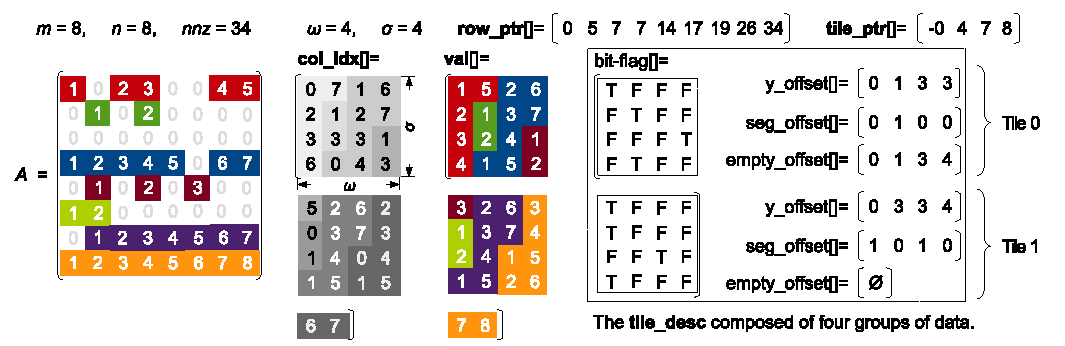
\includegraphics[scale=0.7]{static/A_csr5.pdf}
    \caption{Matrix A stored in CSR5 format (Source:~\cite{liu2015csr5}).}
\end{figure}

Section~\ref{csr5:spmv} outlines the algorithm for performing parallel SpMV using matrices stored in CSR5 format.


\chapter{Implementation}\label{impl}

This chapter introduces \csre{dim}. \csre{dim} is a library/toolkit which is the result of the research done for this
thesis. \csre{dim} is implemented in C++20 using OpenMP and MPI introduced in Sections~\ref{tech:omp} and
~\ref{tech:mpi} respectively.

While the implementation supports COO and CSR as storage formats for sparse matrices, the main storage
format used is CSR5 described in Section~\ref{impl:csr5}. The SpMV algorithm for matrices stored in CSR5
format, introduced in~\cite{liu2015csr5} is further described in Section~\ref{csr5:spmv}.

Lastly, an efficient on-disk storage format used by MATLAB for CSR matrices, storing the matrices in
binary format using HDF5, described in Section~\ref{impl:matlabComp} and its extension to support
matrices stored in CSR5 is outlined in Section~\ref{csr5:onDisk}.

\section{CSR5}\label{impl:csr5}

A common issue of parallel SpMV is load balancing. Storing matrices in CSR5 format avoids this by
grouping data into tiles of a fixed size. Furthermore, the tiles are independent, allowing for a high
degree of parallelism and small critical sections. For this reason \csre{dim}, stores all matrices in
CSR5 format and implements sparse vector multiplication algorithm introduced in~\cite{liu2015csr5}.

Since the implementation of CSR5 SpMV in \csre{dim} utilizes AVX2 instructions, it has some preconditions.
Namely alignment of data passed to the AVX2 intrinsics. Most AVX2 instructions either require data to be
aligned on a 32-byte address or have significantly worse performance for unaligned data.

To facilitate this, C++ offers a customization point in its own contiguous data container \csre{std::vector}.
By specifying an allocator, which returns allocated addresses with a specified alignment as the second
template argument, the implementation can retain the interface of vector and satisfy preconditions of
AVX2 instructions. Any usage of \csre{vector} in this thesis in code examples will refer to a \csre{std::vector}
with a custom-aligned allocator.

\subsection{In memory layout}

As described in~\ref{csr5Intro}, CSR5 storage format, retains the original three arrays of CSR, with
\textbf{column index} and \textbf{values} being in-place transposed. This forms the first part of
CSR5 structure in dim.

The CSR5 structure is templated on floating point type it should use to represent values,
as well as on unsigned type used to represent indices. It also uses concepts, a feature introduced in
C++20, to ensure the passed in types satisfy these constraints. With plain \csre{typename},
the UnsignedType could be an \csre{int} or \csre{FloatingType} a \csre{std::string} and the compiler
would only produce an error if a substitution failed. It is also templated on \csre{Sigma} and \csre{Omega},
the two tuning parameters of CSR5, passed in as non-type template parameters. The defaults are
\csre{FloatingType = double}, \csre{Sigma = 16}, \csre{Omega = 4} and \csre{UnsignedType = uint32_t}.
This limits the size of matrix to be \(2^{32}\times2^{32}\) but can be easily changed to \csre{uint64_t} or
another type if storage for a bigger matrix is required.

\begin{figure}[htp]
    \begin{minted}{C++}
    template<std::floating_point FloatingType = double,
             size_t Sigma = 16,
             size_t Omega = 4,
             std::unsigned_integral UnsignedType = uint32_t>
    struct csr5 {
        // same as CSR.
        UnsignedType         num_cols;
        vector<FloatingType> vals;
        vector<UnsignedType> col_idx;
        vector<UnsignedType> row_ptr;
        // explained in following section.
        csr5_info            csr5_info;
    };
    \end{minted}
    \caption{Pseudo-code for structure holding CSR5 matrix}
\end{figure}

\section{CSR5 info}

\csre{csr5_info} structure contains CSR5 specific information, introduced in~\ref{csr5Intro}.
Namely, \textbf{tile pointer}, \textbf{tile descriptor} and optionally \textbf{empty offset pointer} and
\textbf{empty offset} arrays. Each of these will be explained in a separate section.

\subsection{Tile pointer}

The tile pointer array contains the index of the row of the first element. It works similarly to a CSR
\textbf{row pointer}. The range of rows covered by a tile is obtained by querying \csre{tile_ptr[tid]}
and \csre{tile_ptr[tid + 1]} for the first and last rows respectively (range is open from the top).

The most significant bit of the tile pointer, used as a flag, is set if a tile is \textbf{dirty}.
A tile is dirty if it contains any empty rows. This flag bit must be stripped when the pointer is used for 
indexing into \textbf{row pointer} array. The pointer is wrapped by a structure with \csre{is_dirty} and 
\csre{idx} methods to force the call site to specify the required usage explicitly, making the interface 
less error-prone.

\begin{figure}[htp]
    \begin{minted}{C++}
    struct tile_ptr {
        bool is_dirty();
        UnsignedType raw(); 
        UnsignedType idx(); 
    };
    \end{minted}
    \caption{Tile pointer pseudo-interface}
\end{figure}



\subsection{Tile descriptor}

Amid the new additions to C++20 are bit-manipulation functions in \csre{<bit>} header.
One of the new functions is \csre{std::bit_width} which takes \(N\) and returns \(M\) such that values
up to \(N\) can be stored in \(M\) bits. This function can be used in conjunction with bit-fields
and non-type template parameters to pack descriptors very efficiently while retaining readability when using
them. Since \csre{y_offset} may be at most \(\sigma \cdot \omega\) (the number of new sections is at most the same
as the number of elements in a tile) and \csre{scansum_offset} may be at most \(\omega - 1\) (as it is the number
of empty consecutive columns to the right of current column), the descriptor column and the descriptor
itself can be defined as shown in Figure~\ref{csr5:tileDesc}.

\begin{figure}[htp]

    \begin{minted}{C++}
template<size_t Sigma, size_t Omega>
struct descriptor_column {
    StorageT y_offset: bit_width(Sigma * Omega);
    StorageT scansum_offset: bit_width(Omega);
    StorageT bit_flag: Sigma;
};

template<size_t Sigma, size_t Omega>
struct descriptor {
    descriptor_column<Sigma, Omega> columns[Omega];
};
    \end{minted}
    \caption{Tile descriptor pseudo-code.}\label{csr5:tileDesc}
\end{figure}

As CSR5 tile descriptors contain bit flag maps, \csre{std::popcount} can be used to obtain the number of set bits,
denoting the number of sections started in a column.
Using this function allows the compiler to optimize the call to the instruction of the same name 
if the target ISA supports it.

Previous research about CSR5~\cite{liu2015csr5} concluded, that for modern CPUs with AVX2 extensions, the optimal CSR5 tuning parameters
are \(\sigma = 16\) and \(\omega = 4\).


\subsection{Empty offset}

With \textbf{empty offset} being dependent on number of sections in a tile (and being completely absent
in tiles which \textbf{don't contain empty rows}), it would be inefficient to
store it in the descriptor itself. To avoid too many allocations, two supporting arrays are added.
An \csre{empty_offset_ptr} of size \csre{num_tiles + 1}, which contains offsets for each tile into the
second array, \csre{empty_offset} at which their \csre{empty_offset} array begins.
Thus for each tile, it's empty offset array is defined as
\csre{empty_offset[empty_offset_ptr[i]:empty_offset_ptr[i+1]]}.

The \csre{csr5_info} structure combines these four arrays.


\begin{figure}[htp]
    \begin{minted}{C++}
struct csr5_info {
    vector<tile_ptr>        tile_ptr;
    vector<tile_descriptor> tile_desc;
    vector<UnsignedType>    empty_offset_ptr;
    vector<UnsignedType>    empty_offset;
};
    \end{minted}
    \caption{\csre{csr5_info} pseudo-code.}
\end{figure}

\vfil
\pagebreak

\section{Sparse matrix vector multiplication}\label{csr5:spmv}


\csre{dim} uses CSR5 storage format, described in Section~\ref{csr5Intro}, for sparse matrices. A format purposefully
designed to achieve better performance when performing parallel SpMV\@. This section provides an overview
of this parallel SpMV algorithm (introduced in~\cite{liu2015csr5}) for CSR5 when performed on a multi-threaded
CPU, which supports AVX2 extensions.

\begin{figure}[htp]
    \centering
    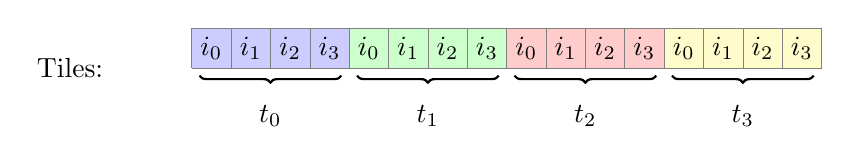
\begin{tikzpicture}
        % tiles

        \coordinate (tileArr) at (0, 0);

        % threads
        \filldraw[blue!20] ($ (tileArr) + (0, 0) $) rectangle ($ (tileArr) + (2, 0.5) $);
        \filldraw[green!20] ($ (tileArr) + (2, 0) $) rectangle ($ (tileArr) + (4, 0.5) $);
        \filldraw[red!20] ($ (tileArr) + (4, 0) $) rectangle ($ (tileArr) + (6, 0.5) $);
        \filldraw[yellow!20] ($ (tileArr) + (6, 0) $) rectangle ($ (tileArr) + (8, 0.5) $);

        \draw[step=0.5cm,gray,very thin] ($ (tileArr) + (0, 0) $) grid ($ (tileArr) + (8, 0.5)$);

        \foreach \x in {0,...,3}
            {
                \coordinate (LLC\x) at ($(tileArr.west) + (\x * 2, 0)$);
                \draw [
                    thick,
                    decoration={
                            brace,
                            mirror,
                            raise=0.1cm
                        },
                    decorate
                ] ($(LLC\x) + (0.1, 0)$) -- ($ (LLC\x) + (2 - 0.1, 0) $)
                node[pos=0.5,below=10pt,black]{$t_\x$};
                \foreach \i in {0,...,3}
                \node at ($(LLC\x) + (\i * 0.5 + 0.25, 0.25)$) {$i_\i$};
            }

        \node[left=of tileArr, anchor=east] {Tiles:};
    \end{tikzpicture}
    \caption{Processing tiles using 4 threads}\label{csr5:thr_dist}
\end{figure}

Using \(N\) threads, each thread gets a contiguous chunk of tiles of the same size (except possibly the
last thread) as shown in Figure~\ref{csr5:thr_dist}. The computational kernel of CSR5 SpMV can be split into three main parts. First each thread processes
its tile chunk. Then the necessary synchronization of sub-results from all threads is performed.
Lastly, the tail partition of the matrix, which was not in any tile (at most \(\sigma{} \cdot \omega\) elements)
is processed.

\begin{algorithm}[h]
    \caption{Corpus of the CSR5 SpMV}
    \begin{algorithmic}
        \Function{spmv}{$\var{A}$, $\var{x}$}
        \State \(\var{y} \gets \text{result vector}\)
        \State \(\var{calib} \gets \mathbbm{0}\)
        \State \(spmv\_full\_tiles(\var{A}, \var{x}, \var{calib}, \var{y})\)
        \State \(spmv\_sync(\var{calib}, \var{y})\)
        \State \(spmv\_tail(\var{A}, \var{x}, \var{y})\)

        \Return $\var{y}$
        \EndFunction
    \end{algorithmic}
\end{algorithm}

\subsection{Processing full tiles}

Each thread processes its assigned tile chunk sequentially.
The notion of \textbf{sub-segments} within a tile column needs
to be established before tile processing can be described.
~\cite{liu2015csr5} defines three types of sub-segments.


\begin{figure}[htp]
    \centering
    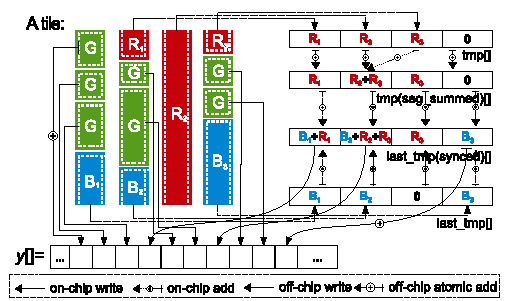
\includegraphics[scale=1]{static/A_secs.pdf}
    \caption{Synchronization of sub-segments within a tile (Source:~\cite{liu2015csr5}).}\label{csr5:tileSync}
\end{figure}

A green sub-segment is a segment that contains
all of the elements of a single row. Meaning, it starts with a set bit in \csre{bit_flag} and ends with
another set-bit (denoting start of a new row) in \csre{bit_flag}. A blue sub-segment is a segment unsealed from
the bottom (column does not end with a set bit in \csre{bit_flag}).
Red sub-segments are segments unsealed from the top (column does not start with a set bit in \csre{bit_flag}).
A tile column with no set bits is also marked as a red segment.
Green sub-segments require no further synchronization. Their sum can be written to the result vector \(y\)
directly by combining \csre{tile_ptr} and \csre{y_offset} information. Red and blue sub-segment sub results must
be synchronized as they do not form a complete segment.


\begin{algorithm}[h]
    \caption{Processing assigned tile chunk CSR5 SpMV}
    \begin{algorithmic}
        \Function{spmv\_full\_tiles}{$\var{A}$, $\var{x}$, $\var{calib}$, $\var{y}$}

        \For{\(\var{tile\_id} \in \text{assigned tiles}\)}
        \State $\var{row} \gets \var{A.tile\_ptr[tile\_id]}$
        \State $\var{desc} \gets \var{A.tile\_desc[tile\_id]}$
        \State $\var{direct} \gets \var{desc}\text{ starts with red sub-segment}$
        \State $spmv\_single\_tile(\var{A}, \var{desc})$
        \If{\(\text{first tile in assigned tiles }\textbf{and}\var{ !direct}\)}
        \State $\var{calib[tid]} \gets \text{first output element}$
        \Else
        \If{\var{direct}}
        \State $\var{y[row]} \gets \text{first output element}$
        \Else
        \State $\var{y[row]} \pluseq \text{first output element}$
        \EndIf
        \EndIf
        \EndFor
        \EndFunction
    \end{algorithmic}
\end{algorithm}

Each tile having 4 columns (\(\omega{}\)) and 16 rows (\(\sigma{}\)), the
thread will perform \(\sigma{}\) iterations,
processing \(\omega{}\) non-zero elements in each iteration using SIMD instructions, in other words,
each column is assigned a SIMD-lane and processed in parallel. This is the reason
for \(\omega{} = 4\) as AVX2 instructions can work on 4 double precision floating point numbers at once
as well as the reason for data being in-place transposed. Algorithm~\ref{csr5:spmv:single_tile} shows
how a single tile column is processed.

\begin{algorithm}[h]
    \caption{Single tile column processing CSR5 SpMV}\label{csr5:spmv:single_tile}
    \begin{algorithmic}
        \Function{spmv\_single\_tile}{$\var{A}$, $\var{desc}$}

        \State $\var{any\_segment} \gets \var{desc.bit\_flag[0]}$

        \State $\var{sum} \gets \var{tile\_vals[0]} \cdot \var{x[tile\_col\_idx[0]]}$
        \State $\var{red\_segsum} \gets 0$

        \For{\(\var{tile\_row} \in range(1, \sigma{})\)}
        \State $\var{segment\_end} \gets \var{desc.bit\_flag[tile\_row]}$
        \If{\var{segment\_end}}
        \If{\var{any\_segment}}
        \State $\text{store to y, green segment}$
        \Else
        \State $\var{red\_segsum} \gets \var{sum}$
        \EndIf

        \State $\var{sum} \gets 0$

        \State $\var{any\_segment} \gets \var{true}$
        \EndIf

        \State $\var{sum} \pluseq \var{tile\_vals[tile\_row]} \cdot \var{x[tile\_col\_idx[tile\_row]]}$
        \EndFor
        \State ${}$ \Comment{Here, \var{sum} will hold the blue sub-segment and \var{red\_segsum} will hold the red sub-segment partial results.
            Except when no no segment has started (\var{any\_segment} is false), then \var{sum} holds the red-subsegment
            partial result and there is no blue sub-segment. The synchronization between lanes is shown in Figure~\ref{csr5:tileSync}.}
        \EndFunction
    \end{algorithmic}
\end{algorithm}


\subsection{Synchronizing overlapping elements}

CSR5 SpMV minimizes the critical sections. The tiles within the chunk assigned to a thread do not have to be
synchronized since they are processed sequentially in the context of the owning thread. Only a single element of
\(y\) may be overlapping between neighboring chunks of tiles, which only happens if the first tile of the
chunk starts with a red sub-section. Synchronization is a two-step process. First, each thread
stores its first output element in a calibrator during the parallel computation. 
Second, after the parallel part of the algorithm is over, each threads calibrator is added to the result 
to perform the final synchronization.

\begin{algorithm}
    \caption{Synchronizing the overlapping elements in y CSR5 SpMV}
    \begin{algorithmic}
        \Function{spmv\_sync}{$\var{calib}$, $\var{y}$}

        \For{\(\var{tid} \in \text{threads}\)}
        \State $\var{y\_idx} \gets \text{tile\_ptr of first tile assigned to thread}$
        \State $\var{y[y\_idx]} \pluseq \var{calib[tid]}$
        \EndFor
        \EndFunction
    \end{algorithmic}
\end{algorithm}

\subsection{Tail partition}

If the number of non-zero elements for a matrix isn't divisible by \(\sigma{} \cdot \omega{}\), there
is a ``tail'' partition which does not form a full tile. The algorithm introduced in Section~\ref{smsf:csr} 
for CSR matrices is used to process this tail partition.

\section{Selecting on disk storage format}\label{impl:matlabComp}

The matrices for which parallelized (and distributed) matrix-vector multiplication has the biggest benefit,
have large on-disk size. This section compares Matrix Market Exchange Format~\cite{mmef} introduced in
Section~\ref{theory:MMEF} and HDF5 backed format
introduced by Matlab 7.3 for storing sparse matrices, comparing both on-disk size and throughput
measured by the number of elements loaded in a second.

\subsection{Matrix Market storage format}

Matrix Market exchange format is designed to be easy to parse. It provides a library to parse
the header and matrix dimensions~\cite{mmC}.
The numerical entries need to be parsed manually, for which most implementations use variations of \texttt{scanf}.
Initial implementation in dim used \texttt{scanf} as well. However, this proved to be a bottleneck as
the average throughput was only \num{4515017} elements/s. Profiling has shown that parsing the string representation
was the most computationally intensive step as 97.89\% of time spent was in \texttt{scanf} itself.
To improve the loading times, to
shorten the iteration times the process of benchmarking, an implementation using
\mintinline{C++}{scnlib}\footnote{\mintinline{C++}{scnlib} is a modern C++ alternative to \texttt{scanf}.}
was created. With an average throughput of \num{6068194} elements/s it resulted in 1.34x speed up, which was
still a major development bottleneck.

\begin{figure}[!h]
    \centering
    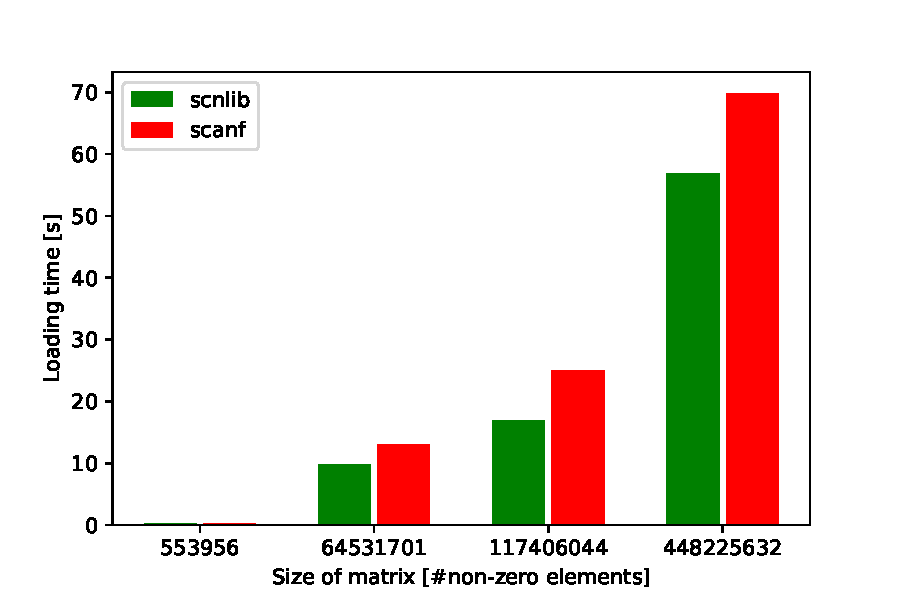
\includegraphics[scale=0.7]{static/mmef_loading.pdf}
    \caption{Loading times of MMEF}
\end{figure}

% TODO: maybe cite matlab and PETSc.
\subsection{Matlab compatible HDF5 sparse matrix storage}

\colorlet{hdtsc}{red!60!yellow}
\colorlet{hdatc}{green!60!gray}
\newcommand{\hdts}[1]{\textcolor{hdtsc}{#1}}
\newcommand{\hdat}[1]{\textcolor{hdatc}{#1}}

Loading matrices stored in binary format using HDF5 introduced in~\ref{theory:HDF5} is supported by MATLAB,
as well as PETSc\footnote{PETSc has to be configured with HDF5 support when it is built}.
They are stored in CSR format, represented as a single HDF5 group containing 3 datasets:
\begin{itemize}
    \item \hdts{data} - values of elements.
    \item \hdts{aj} - column index.
    \item \hdts{ir} - row pointer.
\end{itemize}
And a single attribute \hdat{MATLAB\_sparse} containing the number of columns
of the stored matrix.

\newtcolorbox{infobox}[1][]{%
    enhanced,
    left=2pt,
    nobeforeafter,
    width=0.2\textwidth,
    colback={white!30!yellow},
    box align=center,
    baseline=3.5mm,
    colframe=black,
    #1
}

\begin{figure}[!h]
    \begin{tcolorbox}[title=/A, colback=gray!30!white]
        \begin{infobox}[colback=hdtsc]
            data
        \end{infobox}
        \begin{infobox}[colback=hdtsc]
            aj
        \end{infobox}
        \begin{infobox}[colback=hdtsc]
            ir
        \end{infobox}
        \begin{infobox}[colback=hdatc, width=0.35\textwidth]
            MATLAB\_Sparse
        \end{infobox}
    \end{tcolorbox}
    \caption{Layout of a sparse matrix stored as a HDF5 group}
\end{figure}

Storing the matrices in this format yielded a throughput of \num{110005843} elements/s which is 24.36x speedup
over \texttt{scanf} based implementation of reading matrices stored in Matrix Market Exchange Format
and 18.12x speedup over \texttt{scnlib} implementation.

\begin{figure}[htp]
    \centering
    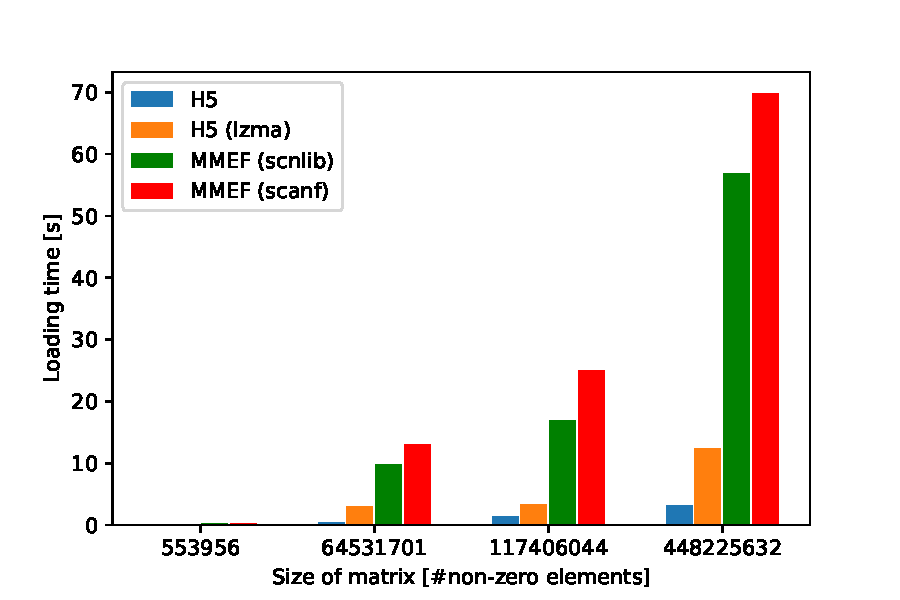
\includegraphics[scale=0.65]{static/mmef_vs_h5.pdf}
    \caption{Load times of HDF5 and MMEF storage formats.}\label{impl:stor:speed}
\end{figure}


Since MMEF uses the coordinate format to store sparse matrices, it may omit elements from symmetrical matrices, which can be inferred
from their symmetrical counterparts. This fact can be used as size optimization. Matrices 2, 3 and 4 in Figure~\ref{impl:stor:size}
are symmetrical. Thus their on-disk size can be smaller with MMEF compared to HDF5.

\begin{figure}[htp]
    \centering
    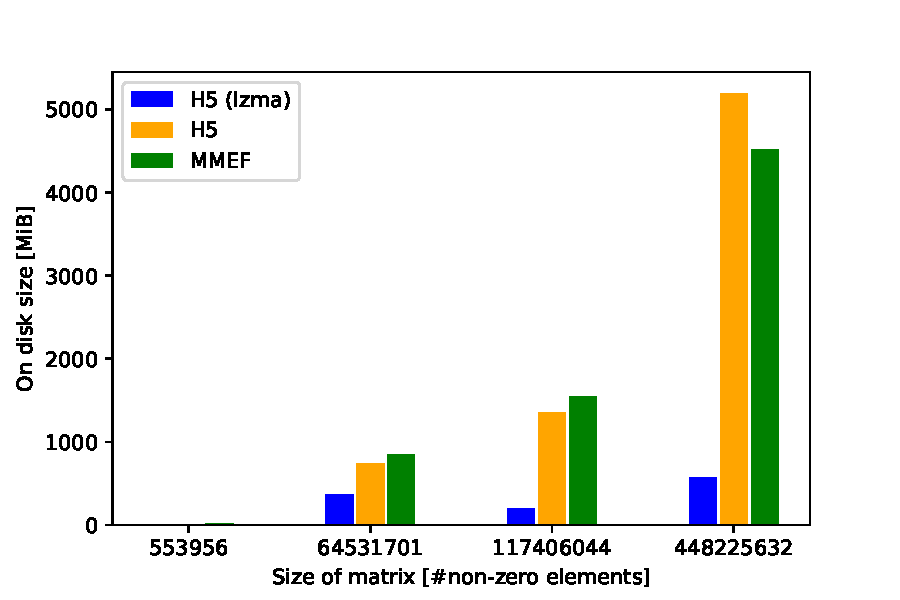
\includegraphics[scale=0.7]{static/mmef_vs_h5_stor.pdf}
    \caption{On-disk size of HDF5 and MMEF storage formats.}\label{impl:stor:size}
\end{figure}

However, the HDF5 format supports dataset compression by LZMA. Setting chunk size to 4096 and compression level to 5 for each of the three datasets,
it is possible to achieve considerable storage savings (the largest matrix is 7.8x smaller stored as compressed HDF5 compared to MMEF)
while maintaining better loading performance, with average throughput being \num{27074837} elements/s, about 4x slower than HDF5 with no compression,
but still 4 and 6 times faster than \texttt{scnlib} and \texttt{scanf} implementations respectively.


\section{On disk storage for CSR5 matrices}\label{csr5:onDisk}

With HDF5 proving to be the faster alternative to textual MMEF format, it is also used for storing sparse
matrices in CSR5 format.

Each of the sequential data members \hdts{row\_ptr}, \hdts{col\_idx}, \hdts{vals}, \hdts{tile\_ptr},
\hdts{empty\_offset}, \hdts{empty\_offset\_ptr}, are stored as one dimensional datasets of same name
and same datatype\footnote{\csre{H5T_STD_U32LE} for all the index arrays and \csre{H5T_IEEE_F64LE} for values}.
\hdat{num\_cols} is stored as an attribute.

\begin{figure}[!h]
    \begin{tcolorbox}[title=/A, colback=gray!30!white]
        \begin{infobox}[colback=hdtsc]
            vals
        \end{infobox}
        \begin{infobox}[colback=hdtsc]
            row\_ptr
        \end{infobox}
        \begin{infobox}[colback=hdtsc]
            col\_idx
        \end{infobox}
        \begin{infobox}[colback=hdtsc, width=0.3\textwidth]
            empty\_offset\_ptr
        \end{infobox}
        \begin{infobox}[colback=hdtsc]
            tile\_ptr
        \end{infobox}
        \begin{infobox}[colback=hdtsc]
            empty\_offset
        \end{infobox}
        \begin{infobox}[colback=hdtsc]
            tile\_desc
        \end{infobox}
        \begin{infobox}[colback=hdatc, width=0.2\textwidth]
            num\_cols
        \end{infobox}
    \end{tcolorbox}
    \caption{Layout of a sparse matrix stored as a HDF5 group}
\end{figure}

\hdts{tile\_desc} is stored as a one-dimensional dataset, with datatype being
an array of 4 little-endian unsigned 32-bit integers. In essence, storing the data to the HDF5 file as
they appear in memory. This decision does put a soft requirement on the code storing the CSR5 matrix to a file
and the code loading it compiled by the same version of a compiler, as
the bit-field in-memory layout is implementation-defined but allows faster loading. Furthermore, both
Clang and GCC implement this in the same way so the requirement is only a soft one, as compatibility can
be easily tested.



\chapter{Distributed Sparse Matrix Vector Multiplication}

Using the principles described in Section~\ref{csr5:spmv}, sparse matrix-vector multiplication can be
distributed across multiple processes. The tiles are first divided among processes as they would be
among threads in a single process implementation (see Figure~\ref{csr5:thr_dist}). Then, these chunks
assigned to processes are further subdivided among the threads of each process. Furthermore, the same
synchronization principles apply, thus only processes that have the first tile starting with red-subsegment
(as defined in~\ref{csr5:spmv}) need to synchronize with the process to the
left\footnote{In the sense of MPI topology.}. This implementation will be referred to as D-CSR5.

Section~\ref{dspmv:load} outlines the algorithm used to load the chunks for each process using HDF5 and
MPI-IO. Then, the synchronization algorithm for edge elements of the result vector as well as an algorithm for
distributing the result vector amongst the processes is introduced in~\ref{dspmv:sync}.



\section{Loading the matrices}\label{dspmv:load}

Since CSR5 partitions the non-zero elements of a matrix into tiles of
size \(\sigma \cdot \omega\), each node can load only data relevant for tiles
assigned to it. This is enabled by two features of HDF5, the first of which
is reading hyperslabs. A hyperslab is a subset of an HDF5 dataset, so
nodes do not have to read whole datasets.

The second feature enabling this is HDF5s ability to utilize MPI-IO, allowing concurrent
reads from every process rather than reading the matrix in the main process
and distributing it amongst the rest of the processes. This imposes a minor limitation
on how the matrix can be stored, or rather how the dataset needs to be structured.
Since MPI-IO was introduced in MPI revision 2.0~\cite{mpi20} in 1997, its API takes
the size of data to be read as an integer argument, thus limiting the maximum amount of data read
in a single call to 2GiB. The dataset needs to be chunked to avoid exceeding this limit
\footnote{experimentally, chunks of 1000000 elements or ~8MiB of double-precision floating-point numbers performed best}, 
else HDF5 tries to read all of it at once, resulting in an error in MPI-IO.


The first step of loading a CSR5 matrix is obtaining the number of tiles of the matrix. This can be
done by querying the dimensions of \csre{tile_desc} dataset, which contains a descriptor for each tile.
The number of tiles is then divided by the number of processes, meaning every process gets equal
number of tiles (bar the last process, which can have less), which in turn means equal number
of non-zero elements.


\begin{algorithm}
    \caption{Computing partition size for each process}
    \begin{algorithmic}
        \Function{calculate\_partition}{$\var{tile\_count}$, $\var{proc\_id}$, $\var{proc\_count}$}
        \State $\var{partition\_size} \gets \lceil\frac{\var{tile\_count}}{\var{proc\_count}}\rceil$
        \State \(\var{first} \gets \var{partition\_size} \cdot \var{proc\_id}\)
        \State $\var{count} \gets min(\var{partition\_size}, \var{tile\_count} - \var{first})$

        \Return $(\var{first}, \var{count})$
        \EndFunction
    \end{algorithmic}
\end{algorithm}

Then, tile descriptors from \csre{tile_desc} dataset, tile pointers from \csre{tile_ptr}
dataset and empty offsets pointers from \csre{tile_desc_offset_ptr} can be loaded.
Sizes of slabs are $\#tiles_{proc}$, $\#tiles_{proc} + 1$ and $\#tiles_{proc} + 1$
respectively, as \csre{*_ptr} datasets use $n+1^{st}$ element to denote end of values
belonging to $n^{th}$ element. Lastly empty offsets from \csre{tile_desc_offset}
are loaded. This forms complete information about CSR5 tiles, and as such, it is
stored in a separate structure named \csre{csr5_info}. This information is useful
even on its own, for example queries about a certain tile, matrix element or row
of matrix and its parent tile can be made just with this information.

\begin{algorithm}
    \caption{Loading CSR5 info}
    \begin{algorithmic}
        \Function{load\_csr5\_info}{$\var{datasets}$, $\var{first}$, $\var{count}$}
        \State $\var{tile\_desc} \gets \var{datasets["tile\_desc"][first:count]}$
        \State $\var{tile\_ptr} \gets \var{datasets["tile\_ptr"][first:count+1]}$
        \State $\var{empty\_off\_ptr} \gets \var{datasets["empty\_offset\_ptr"][first:count+1]}$
        \State $\var{empty\_off} \gets \var{datasets["empty\_offset"][e\_ptr[0]:e\_ptr[-1]]}$
        \EndFunction
    \end{algorithmic}
\end{algorithm}

Lastly, slab of \csre{row_ptr} is loaded, starting at \csre{tile_ptr[0]} and
ending at last output row of chunk of this matrix. This varies, if it is the last
process, the last output row is simply last row of the matrix. For every other tile,
\csre{y_index} in last column + number of bits set in the bit flag of last column
(equal to number of started rows) gives relative offset, which, when added to
\csre{tile_ptr} of the tile will result in absolute offset in y where next row would be.
This model maps onto C++ iterator model, where \csre{end} denotes
element one past the end of the range. With this information, \csre{row_ptr} can be
loaded. Since, \csre{row_ptr} has the same meaning as in CSR, hyperslabs for
values from \csre{vals} dataset, and column indices from \csre{col_idx} dataset
are both starting at \csre{row_ptr[0]} and ending at \csre{row_ptr[-1]}.


\begin{algorithm}
    \caption{Loading CSR data}
    \begin{algorithmic}
        \Function{last\_out\_idx}{}
        \State \(\var{lid} \gets \text{`last tile id'}\)
        \State \(\var{last\_desc} \gets \var{tile\_desc[lid]}\)
        \State \(\var{secs\_starting} \gets popcount(\var{last\_desc[lid].bit\_flag})\)
        \State \(\var{rel\_off} \gets \var{last\_desc[lid].y\_index + secs\_starting}\)

        \If{\(dirty(\var{last\_desc})\)}
        \State \(\var{empty\_start} \gets \var{empty\_off\_ptr[lid]}\)
        \State \(\var{rel\_off} \gets \var{empty\_off[empty\_start + rel\_off]}\)
        \EndIf

        \Return \(\var{tile\_ptr[lid] + relative\_offset}\)
        \EndFunction

        \Function{load\_csr\_data}{$datasets$, $first$, $count$}
        \State \(\var{fr\_id} \gets \var{tile\_ptr[0]}\)
        \State \(\var{lr\_id} \gets last\_out\_idx()\)
        \State \(\var{row\_ptr} \gets \var{datasets["row\_ptr"][fr\_id:lr\_id]}\)
        \State \(\var{values} \gets \var{datasets["vals"][row\_ptr[0]: row\_ptr[-1]]}\)
        \State \(\var{col\_idx} \gets \var{datasets["col\_idx"][row\_ptr[0]: row\_ptr[-1]]}\)
        \EndFunction
    \end{algorithmic}
\end{algorithm}

\section{Synchronization}\label{dspmv:sync}

As explained in~\ref{csr5:spmv} a tile may share at most one output element with its neighbor,
so a process has to synchronize at most two elements in its output range in \(y\). The synchronization
mechanism is explained in Section~\ref{dspmv:sync}. If all processes need the whole result vector,
it can be distributed as explained by Section~\ref{dspmv:dist}.

To illustrate, let \(A\) be a \(4\times4\) square matrix with 8 non-zero elements, multiplied by a vector
\(x\), while SPmV is distributed across four processes labeled p1-p4 and let \(\sigma = 2\) and \(\omega = 1\).
Thus, each process gets one CSR5 tile containing 2 non-zero elements.

\begin{figure}[htp]
    \centering
    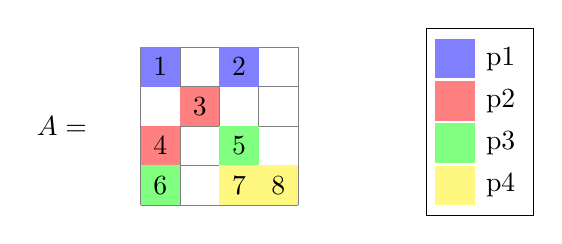
\begin{tikzpicture}[
            p1node/.style={rectangle, fill=blue!50, very thick, minimum size=5mm},
            p2node/.style={rectangle, fill=red!50, very thick, minimum size=5mm},
            p3node/.style={rectangle, fill=green!50, very thick, minimum size=5mm},
            p4node/.style={rectangle, fill=yellow!50, very thick, minimum size=5mm},
        ]

        \coordinate (ACoo) at (0, 0);

        \coordinate (yCoo) at (3 - 0.001, 1 - 0.001);

        \node at ($ (ACoo) + (-1, 1)$) {$A =$};

        % matrix
        \draw[step=0.5cm,gray,very thin] (ACoo) grid ($ (ACoo) + (2,2) $);

        % r0
        \node[p1node] at ($ (ACoo) + (0.25, 1.75) $) {1};
        \node[p1node] at ($ (ACoo) + (1.25, 1.75) $) {2};

        %r1
        \node[p2node] at ($ (ACoo) + (0.75, 1.25) $) {3};

        %r2
        \node[p2node] at ($ (ACoo) + (0.25, 0.75) $) {4};
        \node[p3node] at ($ (ACoo) + (1.25, 0.75) $) {5};

        %r3
        \node[p3node] at ($ (ACoo) + (0.25, 0.25) $) {6};
        \node[p4node] at ($ (ACoo) + (1.25, 0.25) $) {7};
        \node[p4node] at ($ (ACoo) + (1.75, 0.25) $) {8};


        \matrix [draw,below left] at (5, 2.25) {
            \node [p1node,label=right:p1] {}; \\
            \node [p2node,label=right:p2] {}; \\
            \node [p3node,label=right:p3] {}; \\
            \node [p4node,label=right:p4] {}; \\
        };
    \end{tikzpicture}
    \caption{Distribution of $A$ across 4 processes}
\end{figure}



\subsection{Synchronizing overlapping output ranges}\label{dspmv:syncOver}

Let \textbf{output index} be an index into result vector $y$ of sparse matrix vector
multiplication $Ax = y$ and \textbf{output range} be a pair of output indices, denoting
first and last output index for each process.

\begin{figure}[htp]
    \centering
    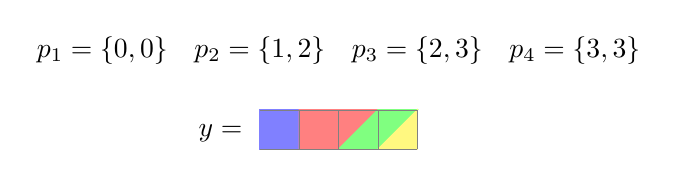
\begin{tikzpicture}[
            p1node/.style={rectangle, fill=blue!50, very thick, minimum size=5mm},
            p2node/.style={rectangle, fill=red!50, very thick, minimum size=5mm},
            p3node/.style={rectangle, fill=green!50, very thick, minimum size=5mm},
            p4node/.style={rectangle, fill=yellow!50, very thick, minimum size=5mm}
        ]

        \node at (0, 0.75) {$p_1 = \{0, 0\}$};
        \node at (2, 0.75) {$p_2 = \{1, 2\}$};
        \node at (4, 0.75) {$p_3 = \{2, 3\}$};
        \node at (6, 0.75) {$p_4 = \{3, 3\}$};

        \coordinate (yCoo) at (2, -0.5);
        \node at ($ (yCoo) + (-0.5, 0.2) $) {$y = $};


        % p1 output
        \filldraw[blue!50] (yCoo) rectangle ($ (yCoo) + (0.5, 0.5)$);

        % p2 output
        \filldraw[red!50] ($(yCoo) + (0.5, 0) $) -- ($(yCoo) + (1, 0) $) -- ($ (yCoo) + (1.5, 0.5)$) -- ($ (yCoo) + (0.5, 0.5)$) -- cycle;

        % p3 output
        \filldraw[green!50] ($(yCoo) + (1, 0) $) -- ($(yCoo) + (1.5, 0) $) -- ($ (yCoo) + (2, 0.5)$) -- ($ (yCoo) + (1.5, 0.5)$) -- cycle;

        % p4 output
        \filldraw[yellow!50] ($(yCoo) + (1.5, 0) $) -- ($(yCoo) + (2, 0) $) -- ($ (yCoo) + (2, 0.5)$)-- cycle;

        \draw[step=0.5cm,gray,very thin] (yCoo) grid ($ (yCoo) + (2 + 0.001, 0.5 + 0.001)$);
    \end{tikzpicture}
    \caption{Output ranges for processes p1-p4}
\end{figure}

Neighboring processes may share an output index. In the case of \(Ax = y\) established in the previous section,
\(y_2\) and \(y_3\) are partially computed by processes p2, p3 and p3, p4 respectively. 
An ownership model needs to be defined before the synchronization can be described. 
The process with the lowest rank (in terms of MPI ranks) that writes to an output index 
owns the element of \(y\). Thus \(y_2\) is owned by p2 while \(y_3\) is owned by p3.

\begin{figure}[htp]
    \centering
    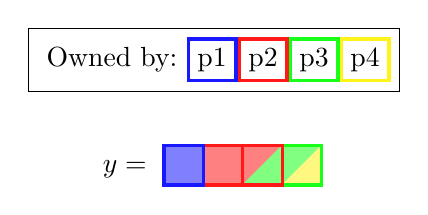
\begin{tikzpicture}[
            p1own/.style={rectangle, draw=blue!90, very thick, minimum size=5mm},
            p2own/.style={rectangle, draw=red!90, very thick, minimum size=5mm},
            p3own/.style={rectangle, draw=green!90, very thick, minimum size=5mm},
            p4own/.style={rectangle, draw=yellow!90, very thick, minimum size=5mm},
        ]

        \coordinate (yCoo) at (0.5 - 0.001, 1 - 0.001);
        \node at ($ (yCoo) + (-0.5, 0.2) $) {$y = $};

        % p1 output
        \filldraw[blue!50] (yCoo) rectangle ($ (yCoo) + (0.5, 0.5)$);

        % p2 output
        \filldraw[red!50] ($(yCoo) + (0.5, 0) $) -- ($(yCoo) + (1, 0) $) -- ($ (yCoo) + (1.5, 0.5)$) -- ($ (yCoo) + (0.5, 0.5)$) -- cycle;

        % p3 output
        \filldraw[green!50] ($(yCoo) + (1, 0) $) -- ($(yCoo) + (1.5, 0) $) -- ($ (yCoo) + (2, 0.5)$) -- ($ (yCoo) + (1.5, 0.5)$) -- cycle;

        % p4 output
        \filldraw[yellow!50] ($(yCoo) + (1.5, 0) $) -- ($(yCoo) + (2, 0) $) -- ($ (yCoo) + (2, 0.5)$)-- cycle;

        \draw[step=0.5cm,gray,very thin] (yCoo) grid ($ (yCoo) + (2 + 0.001, 0.5 + 0.001)$);

        \node[p3own] at ($(yCoo) + (1.75, 0.25)$) {};
        \node[p2own] at ($(yCoo) + (1.25, 0.25)$) {};
        \node[p2own] at ($(yCoo) + (0.75, 0.25)$) {};
        \node[p1own] at ($(yCoo) + (0.25, 0.25)$) {};

        \matrix [draw,below left] at ($(yCoo) + (3, 2)$) {
            \node {Owned by:};  &
            \node [p1own] {p1}; &
            \node [p2own] {p2}; &
            \node [p3own] {p3}; &
            \node [p4own] {p4};   \\
        };
    \end{tikzpicture}
    \caption{Ownership of \(y\)}
\end{figure}

Each process has two MPI communicators to synchronize the elements. One for synchronizing the element
it owns referred to as OWN, and one for synchronizing the element it does not own referred to as LEFT.
Either of these communicators can be \csre{MPI_COMM_NULL} if no synchronization is necessary for the owned
(or non-owned) element.

The first step in creating synchronization communicators is participating processes exchanging their output ranges.
Output ranges consist of indices of the first and last output elements for each process. From
these, each process can check if it needs to synchronize to the left and if it needs to
create a communicator on which processes to the right of it will sync.

\begin{figure}[htp]
    \centering
    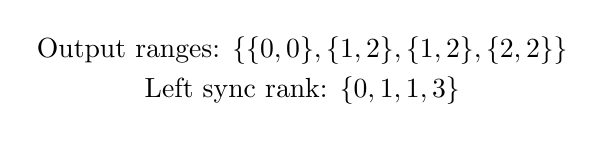
\begin{tikzpicture}
        \node at (0, 0) {Output ranges: $\{\{0, 0\}, \{1, 2\}, \{1, 2\}, \{2, 2\}\}$};
        \node at (0, -0.5) {Left sync rank: $\{0, 1, 1, 3\}$};
    \end{tikzpicture}
    \caption{Pre-computation step of synchronizing \(y\)}
\end{figure}

\csre{MPI_Comm_Split} splits a communicator according to a \csre{color} and a \csre{key}.
\csre{color} is used to group processes, and \csre{key} is used to create ordering within processes
of same \csre{color}. Furthermore, if only a single process is present, the
returned communicator will be \csre{MPI_COMM_NULL}. Thus if all processes first compute the
process which will own the first output index in their output range, then it is possible
to iterate over every rank and allow every process to establish an owning communicator
in the iteration in which \(i = rank\) and for all the processes which need to synchronize
the element this process owns, to register to this communicator. If no process registers,
the communicator returned is \csre{MPI_COMM_NULL}, and no synchronization is performed.

\begin{algorithm}[htp]
    \caption{Creating communicators for syncing edge elements}
    \begin{algorithmic}
        \Function{create\_syncs}{$my\_rank$, $comm\_size$}
        \State $\var{output\_ranges} \gets \text{ranges from all processes}$
        \State $\var{syncs\_to} \gets \var{my\_rank}$
        \State $\var{this\_node\_range} \gets \var{output\_ranges[my\_rank]}$
        \While {$\var{syncs\_to} \neq 0 \AND \text{elements overlap}$} % TODO: latex doesn't like the long condition
        \State $\var{syncs\_to} \gets \var{syncs\_to} - 1$
        \EndWhile

        \For{\var{rank = 0; rank < comm\_size; ++rank}}
        \If{$\var{rank} \equiv \var{my\_rank}$}
        \State $\var{own\_sync} \gets \var{MPI\_Comm\_Split(comm, my\_rank, my\_rank)}$
        \ElsIf{$\var{rank} \equiv \var{syncs\_to}$}
        \State $\var{left\_sync} \gets \var{MPI\_Comm\_Split(comm, syncs\_to, my\_rank)}$
        \Else {}
        \State $\var{MPI\_Comm\_Split(comm, MPI\_UNDEFINED, MPI\_UNDEFINED)}$
        \EndIf
        \EndFor
        \EndFunction
    \end{algorithmic}
\end{algorithm}

Depending on values of LEFT and OWN communicators the processes can be split into 4 categories:

\begin{itemize}
    \item (NULL, NULL) - self-contained, not sharing any output indices (p1).
    \item (NULL, !NULL) - doesn't share first output element (p2).
    \item (!NULL, NULL) - doesn't share last output element (p4).
    \item (!NULL, !NULL) - shares both first and last elements (p3).
\end{itemize}


\begin{figure}[htp]
    \centering
    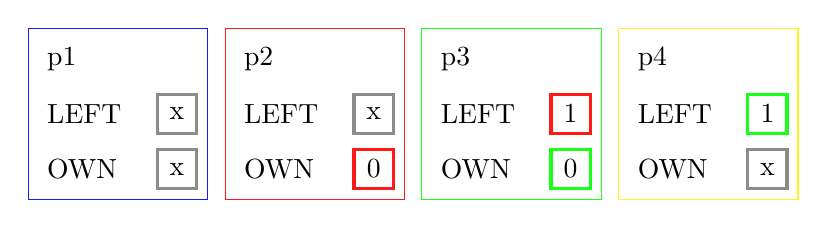
\begin{tikzpicture}[
            node distance=7mm,
            commst/.style={rectangle, very thick, minimum size=5mm, anchor=west},
            tag/.style={minimum size=5mm, anchor=west},
            commstnull/.style={rectangle, very thick, minimum size=5mm, draw=gray!90, anchor=west},
        ]

        \node (p1) {p1};

        \node (p1lt) [below=of p1.west, tag] {LEFT};
        \node (p1l) [right=1.5cm of p1lt.west, commstnull] {x};

        \node (p1ot) [below=of p1lt.west, tag] {OWN};
        \node (p1o) [below=of p1l.west, commstnull] {x};

        \node [draw=blue!90, fit={(p1) (p1lt) (p1l) (p1o)}] {};

        \node (p2) at (2.5, 0) {p2};

        \node (p2lt) [below=of p2.west, tag] {LEFT};
        \node (p2l) [right=1.5cm of p2lt.west, commstnull] {x};

        \node (p2ot) [below=of p2lt.west, tag] {OWN};
        \node (p2o) [below=of p2l.west, commst, style={draw=red!90}] {0};

        \node [draw=red!90, fit={(p2) (p2lt) (p2l) (p2o)}] {};

        \node (p3) at (5, 0) {p3};

        \node (p3lt) [below=of p3.west, tag] {LEFT};
        \node (p3l) [right=1.5cm of p3lt.west, commst, style={draw=red!90}] {1};

        \node (p3ot) [below=of p3lt.west, tag] {OWN};
        \node (p3o) [below=of p3l.west, commst, style={draw=green!90}] {0};

        \node [draw=green!90, fit={(p3) (p3lt) (p3l) (p3o)}] {};

        \node (p4) at (7.5, 0) {p4};

        \node (p4lt) [below=of p4.west, tag] {LEFT};
        \node (p4l) [right=1.5cm of p4lt.west, commst, style={draw=green!90}] {1};

        \node (p4ot) [below=of p4lt.west, tag] {OWN};
        \node (p4o) [below=of p4l.west, commstnull] {x};

        \node [draw=yellow!90, fit={(p4) (p4lt) (p4l) (p4o)}] {};
    \end{tikzpicture}
    \caption{Synchronization communicators}
\end{figure}


With the communicators established, processes that have at least one non-NULL
communicator call \csre{MPI_Allreduce} with either first, last, or both elements
to synchronize the edge elements in every participating process.

\begin{figure}[htp]
    \centering
    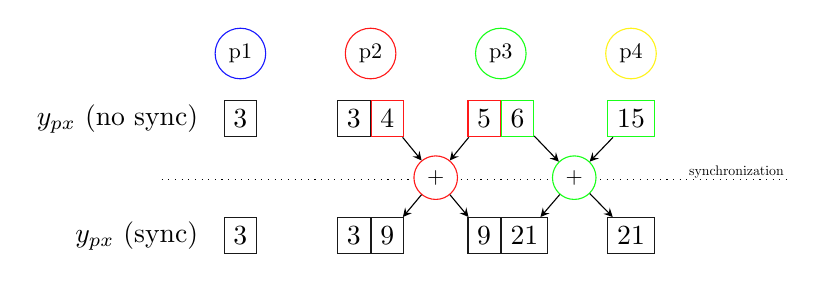
\begin{tikzpicture}[proc/.style={circle, minimum width=5mm, scale=0.8}]
        \node (p1) [proc, style={draw=blue!90}] {p1};
        \node (p2) [right=of p1, proc, style={draw=red!90}] {p2};
        \node (p3) [right=of p2, proc, style={draw=green!90}] {p3};
        \node (p4) [right=of p3, proc, style={draw=yellow!90}] {p4};

        \node (p11) [below=0.5cm of p1, rectangle, draw=black!90, anchor=center] {3};

        \node (p21) [below=0.5cm of p2, rectangle, draw=black!90, anchor=east] {3};
        \node (p22) [right=0cm of p21.east, rectangle, draw=red!90] {4};

        \node (p31) [below=0.5cm of p3, rectangle, draw=red!90,anchor=east] {5};
        \node (p32) [right=0cm of p31.east, rectangle, draw=green!90] {6};

        \node (p41) [below=0.5cm of p4, rectangle, draw=green!90, anchor=center] {15};

        \draw [dotted] (-1, -1.6) -- (7, -1.6);
        \node (st) [scale=0.5] at (6.3, -1.5) {synchronization};

        \node [left=0.2cm of p11, anchor=east] {$y_{px}$ (no sync)};

        \node (r23) [circle, fill=white!100, draw=red!90, minimum width=5mm, scale=0.8, anchor=center] at ($(p22)!0.5!(p31) + (0, -0.75)$) {$+$};
        \node (r34) [circle, fill=white!100, draw=green!90, minimum width=5mm, scale=0.8, anchor=center] at ($(p32)!0.5!(p41) + (0, -0.75)$) {$+$};

        \draw [-stealth] (p22) -- (r23);
        \draw [-stealth] (p31) -- (r23);

        \draw [-stealth] (p32) -- (r34);
        \draw [-stealth] (p41) -- (r34);

        \node (sp11) [below=1.25cm of p11, rectangle, draw=black!90, anchor=center] {3};

        \node (sp21) [below=1.25cm of p21, rectangle, draw=black!90, anchor=center] {3};
        \node (sp22) [below=1.25cm of p22, rectangle, draw=black!90, anchor=center] {9};

        \node (sp31) [below=1.25cm of p31, rectangle, draw=black!90, anchor=center] {9};
        \node (sp32) [right=0cm of sp31, rectangle, draw=black!90, anchor=west] {21};

        \node (sp41) [below=1.25cm of p41, rectangle, draw=black!90, anchor=center] {21};

        \node [left=0.2cm of sp11, anchor=east] {$y_{px}$ (sync)};


        \draw [-stealth] (r23) -- (sp22);
        \draw [-stealth] (r23) -- (sp31);

        \draw [-stealth] (r34) -- (sp32);
        \draw [-stealth] (r34) -- (sp41);



    \end{tikzpicture}
    \caption{Synchronization of result of \(Ax = y\) assuming \(x=\mathbbm{1}\)}
\end{figure}


\subsection{Distributing the result}\label{dspmv:dist}

After synchronizing overlapping output ranges, the result can be distributed to every process.
Ownership rules established in the previous section apply when distributing the result vector.
The first process that writes an element owns it and is the only process broadcasting it to
others.

\begin{figure}[htp]
    \centering
    \begin{tikzpicture}[proc/.style={circle, minimum width=5mm, scale=0.8}]
        \node (p1) [proc, style={draw=blue!90}] {p1};
        \node (p2) [right=of p1, proc, style={draw=red!90}] {p2};
        \node (p3) [right=of p2, proc, style={draw=green!90}] {p3};
        \node (p4) [right=of p3, proc, style={draw=yellow!90}] {p4};

        \node (p11) [below=0.5cm of p1, rectangle, draw=black!90, anchor=center] {3};

        \node (p21) [below=0.5cm of p2, rectangle, draw=black!90, anchor=east] {3};
        \node (p22) [right=0cm of p21.east, rectangle, draw=black!90] {9};

        \node (p31) [below=0.5cm of p3, rectangle, draw=gray!90,anchor=east] {9};
        \node (p32) [right=0cm of p31.east, rectangle, draw=black!90] {21};

        \node (p41) [below=0.5cm of p4, rectangle, draw=gray!90, anchor=center] {21};

        \draw [dotted] (-1, -1.6) -- (7, -1.6);
        \node (st) [scale=0.5] at (6.3, -1.5) {\csre{MPI_Allgatherv}};

        \node [left=0.2cm of p11, anchor=east] {$y_{px}$ (sync)};


        \coordinate (res) at ($(p2)!0.5!(p3) + (0, -2.5)$);

        \node (sp1) [rectangle, draw=blue!90, anchor=center] at ($(res) + (-0.75, 0.25) $) {3};
        \draw [-stealth] (p11) -- (sp1);

        \node (sp2) [right=0cm of sp1.east, rectangle, draw=red!90, anchor=west] {3};
        \draw [-stealth] (p21) -- (sp2);

        \node (sp3) [right=0cm of sp2.east, rectangle, draw=red!90, anchor=west] {9};
        \draw [-stealth] (p22) -- (sp3);

        \node (sp4) [right=0cm of sp3.east, rectangle, draw=green!90, anchor=west] {21};
        \draw [-stealth] (p32) -- (sp4);

        \node [left=0.2cm of sp11, anchor=east] {$y$ (sync)};
    \end{tikzpicture}
    \caption{Distribution of result of \(Ax = y\) assuming \(x=\mathbbm{1}\)}
\end{figure}

Before partial results can be distributed, output ranges must be exchanged (which is done for the edge
element synchronization). From these ranges,
an array of offsets into the complete result vector are computed. Each process
either broadcasts its whole output range or skips the first element of the range if
it is owned by a process to the left. The actual distribution of results is performed by
calling \csre{MPI_Allgatherv}, introduced in Section~\ref{tech:mpi:red}, 
with offsets and sizes computed as explained previously.

\begin{algorithm}[htp]
    \caption{Synchronizing partial results across processes}
    \begin{algorithmic}
        \Function{compute\_offsets}{}
        \State $\var{output\_ranges} \gets \text{ranges from all nodes}$
        \State $\var{recvcounts[0]} \gets \var{output\_ranges[0].count}$
        \State $\var{displs[0]} \gets \var{output\_ranges[0].first\_idx}$

        \For{\var{rank = 1; rank < comm\_size; ++rank}}

        \State $\var{skip\_first} \gets \text{range overlaps}$
        \If{$\var{skip\_first}$}
        \State $\var{output\_ranges[rank].first\_idx} \pluseq 1$
        \EndIf

        \State $\var{recvcounts[rank]} \gets \var{output\_ranges[rank].count}$
        \State $\var{displs[rank]} \gets \var{output\_ranges[rank].first\_idx}$

        \EndFor

        \Return $\var{recvcounts}, \var{displs}$

        \EndFunction

        \Function{sync}{$\var{owned\_partial\_result}$, $\var{full\_result}$, $\var{comm}$}
        \State $\var{displs}, \var{recvcounts} \gets \var{compute\_offsets()}$
        \State $\var{MPI\_Allgatherv(owned\_partial\_result, full\_result, recvcounts, comm)}$

        \EndFunction
    \end{algorithmic}
\end{algorithm}


\chapter{Benchmarks}

To measure real-world performance of distributed sparse matrix-vector multiplication
three implementations of numerical solvers using conjugate gradient method briefly explained in
Appendix~\ref{app:cg}, were produced.
Single and multi process implementations using the \csre{dim} toolkit 
and a \texttt{PETSc} based multi process implementation.

\section{Specification}

Each implementation will load matrix $A$ and perform 100 iterations of conjugate
gradient method, trying to find $x$ satisfying $Ax=\mathbbm{1}$.

Each step of conjugate gradient iteration is kept track of, and the total time
for each step is output in a JSON file.

\subsection{Benchmark data}

Three square matrices were selected for benchmarking.

\begin{tabular}{|c|c|c|c|}
    \hline
    \textbf{name}      & \textbf{n} & $n_{nz}$   & \textbf{CSR5 on-disk size} [GiB] \\
    \hline
    \hline
    \textbf{nlpkkt240} & 27993600   & 774472352  & 9.1                              \\
    \hline
    \textbf{GAP-web}   & 50636151   & 1930292948 & 22.6                             \\
    \hline
    \textbf{GAP-kron}  & 134217726  & 4223264644 & 49.6                             \\
    \hline
\end{tabular}


\subsection{Compilation options}

The benchmarks were run on the RCI cluster, using AMD nodes.

\textbf{CPU}: \texttt{2 x AMD EPYC 7543 (64 cores/128 threads 2.8GHz)} \\
\textbf{Network}: \texttt{200GbE InfiniBand EDR for MPI communication}\\
\begin{minipage}{0.5\textwidth}
    \textbf{RAM}: \texttt{1TB}\\
    \textbf{Storage}: \texttt{8TB NVMe} \\
\end{minipage}%
\begin{minipage}{0.5\textwidth}
    \textbf{Compiler}: \texttt{GCC 10.3} \\
    \textbf{Optimization level}: \texttt{-O3} \\
    \textbf{March}: \texttt{native(znver2)} \\
\end{minipage}



\section{Single process implementation}

Single process implementation uses CSR5 format for storing the sparse matrix and the
SpMV algorithm  described in Section~\ref{csr5:spmv} for the \(A \cdot s\) step. It was ran
with 16, 32, 64, and 128 CPUs available for each input matrix. The naming of steps 
in the graphs follows the naming scheme introduced in Section~\ref{dcg:steps}.

\begin{figure}[htp]
    \centering
    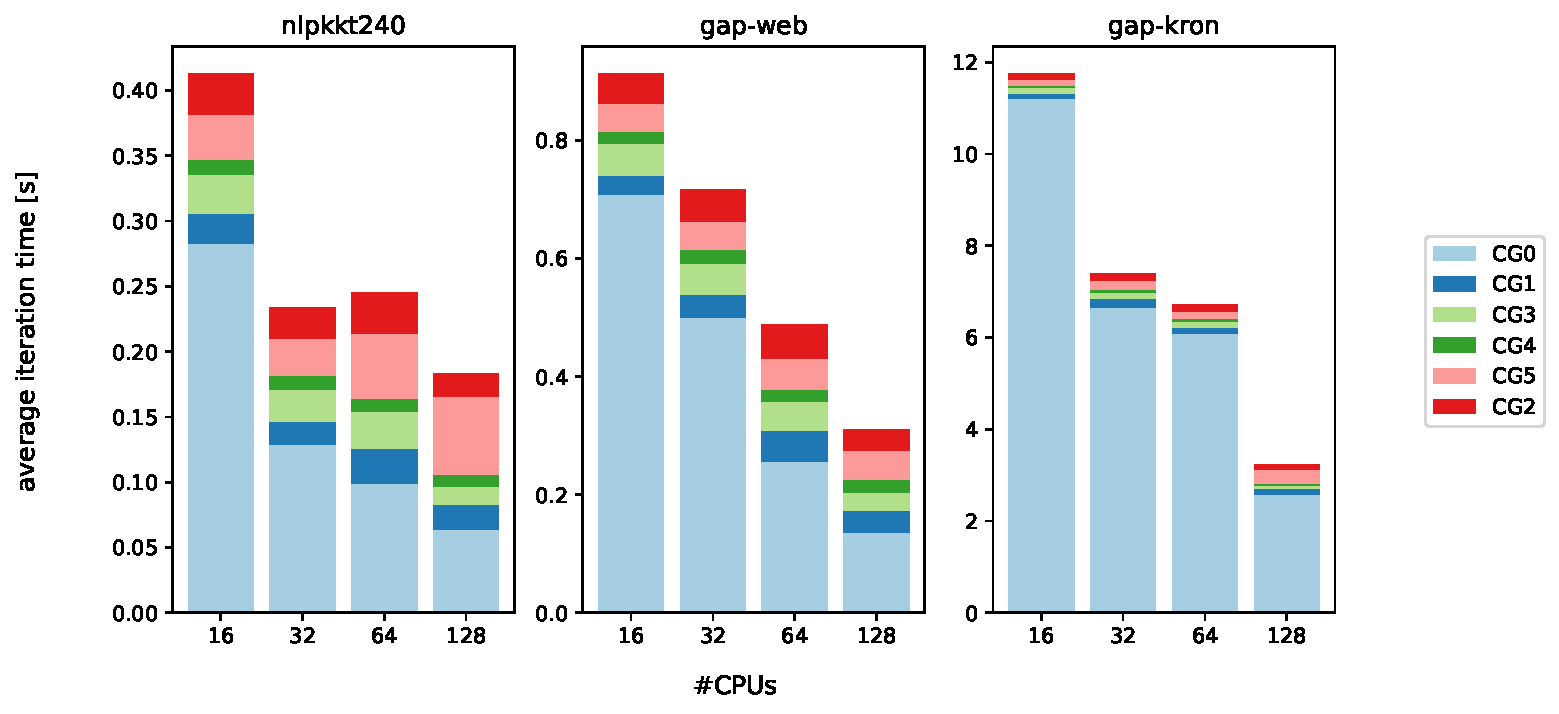
\includegraphics[scale=0.5]{static/single_process.pdf}
    \caption{Scaling of single process implementation CG with CPU count}
\end{figure}

Benchmark results show that the sparse matrix-vector multiplication
\(As\) is the most computationally intensive step as it takes 68.5, 77.5, and 95.4\% of
total iteration time for \textit{nlpkkt240}, \textit{gap-web}, and \textit{gap-kron} 
matrices respectively when the single process implementation is running on 16 threads.


\begin{figure}[htp]
    \centering
    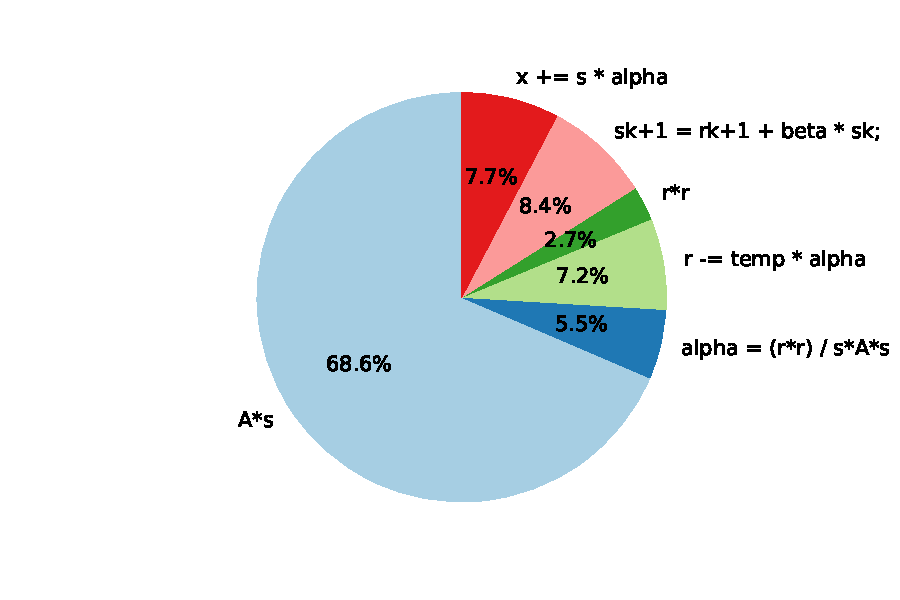
\includegraphics[scale=0.6]{static/cg_sp_nlpkkt240_16.pdf}
    \caption{Percentage of time spent in steps of CG (nlpkkt240, 16CPUs)}
\end{figure}


It can further be observed that sparse matrix-vector multiplication scales well with
number of CPUs available.

\subsection{IO}

With the benchmarked matrices ranging in size from 9GiB up to 50GiB, loading the matrices
may become a non-negligible part of total computation time. The following graphs show the impact of
IO on total run-time of benchmark as well as achieved throughput using the fastest single process
configuration with 128CPUs available.

\begin{figure}[htp]
    \centering
    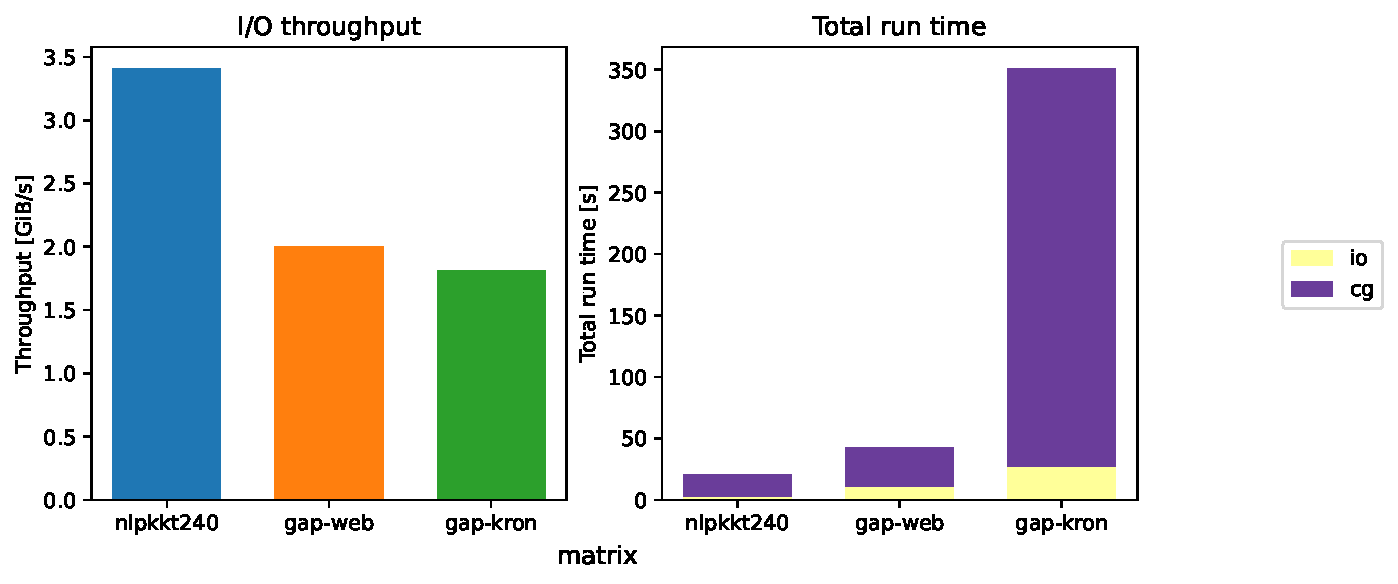
\includegraphics[scale=0.6]{static/io_sp.pdf}
    \caption{Time spent doing IO vs conjugate gradient (128 CPUs used)}
\end{figure}

By using HDF5 to store matrices in binary format and utilizing fast NVMe storage available
on RCI nodes, the impact of IO on total run time can be minimized. However even after doing so,
for \csre{GAP-web} matrix, loading the matrix takes up 26\% of the total benchmark runtime.


\section{Distributed conjugate gradient implementation}

First, three MPI layouts were benchmarked, each totaling 128CPUs. A layout
in this text will mean a triplet of \textbf{node count} $N$,
\textbf{number of processes per node} $P$
and \textbf{number of CPUs per process} $C$ (usually abbreviated to \csre{N-P-C}).
The benchmarked layouts were \csre{2-1-64}, \csre{4-1-32} and \csre{8-1-16}, keeping
the same CPU count as the fastest single process implementation so that the results
can be compared directly.

\begin{figure}[htp]
    \centering
    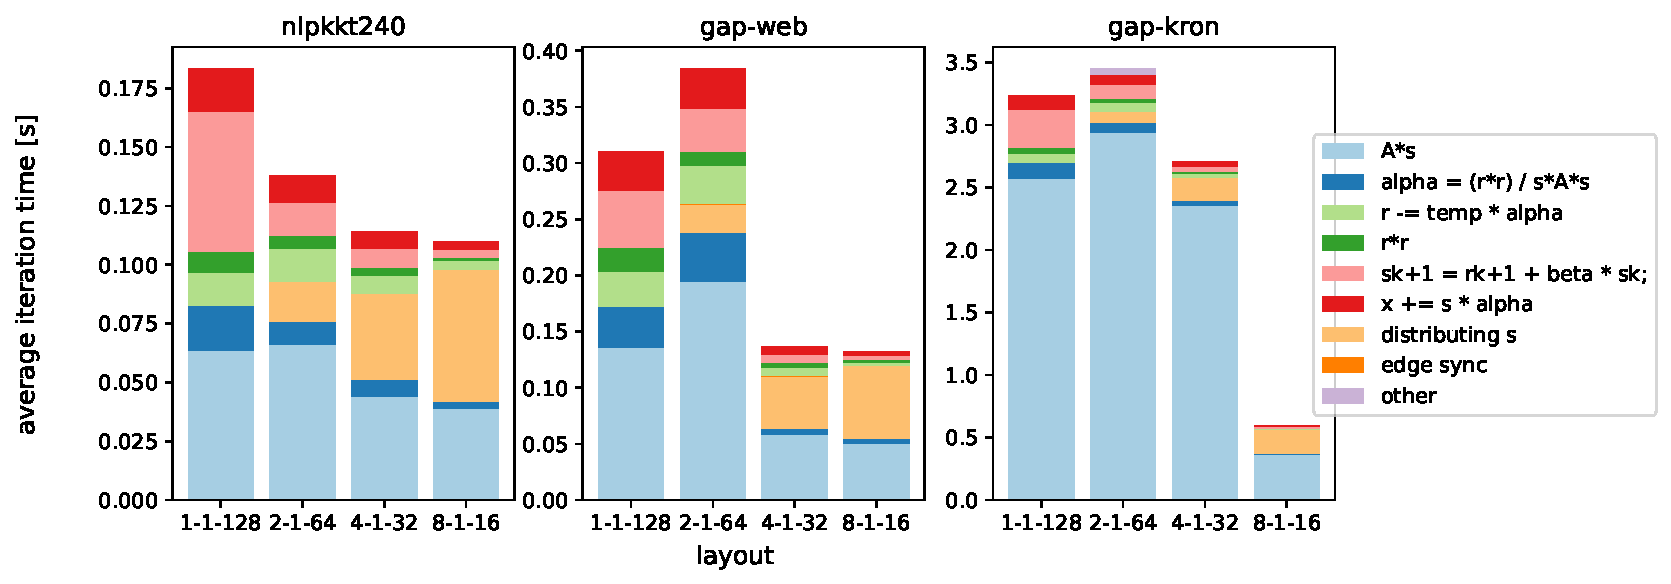
\includegraphics[scale=0.5]{static/mpi.pdf}
    \caption{Average iteration times of single and multi process implementations}
\end{figure}

\subsection{IO}

RCI cluster provides BeeGFS parallel filesystem and by utilizing the algorithm described in
Section~\ref{dspmv:load}, the IO throughput can be improved considerably. Using best-performing \csre{8-1-16}
layout results, throughput has improved by a factor of 2.5, 5.6, and 6.9 for \textit{nlpkkt240}, \textit{gap-web}
and \textit{gap-kron} respectively.

\begin{figure}[htp]
    \centering
    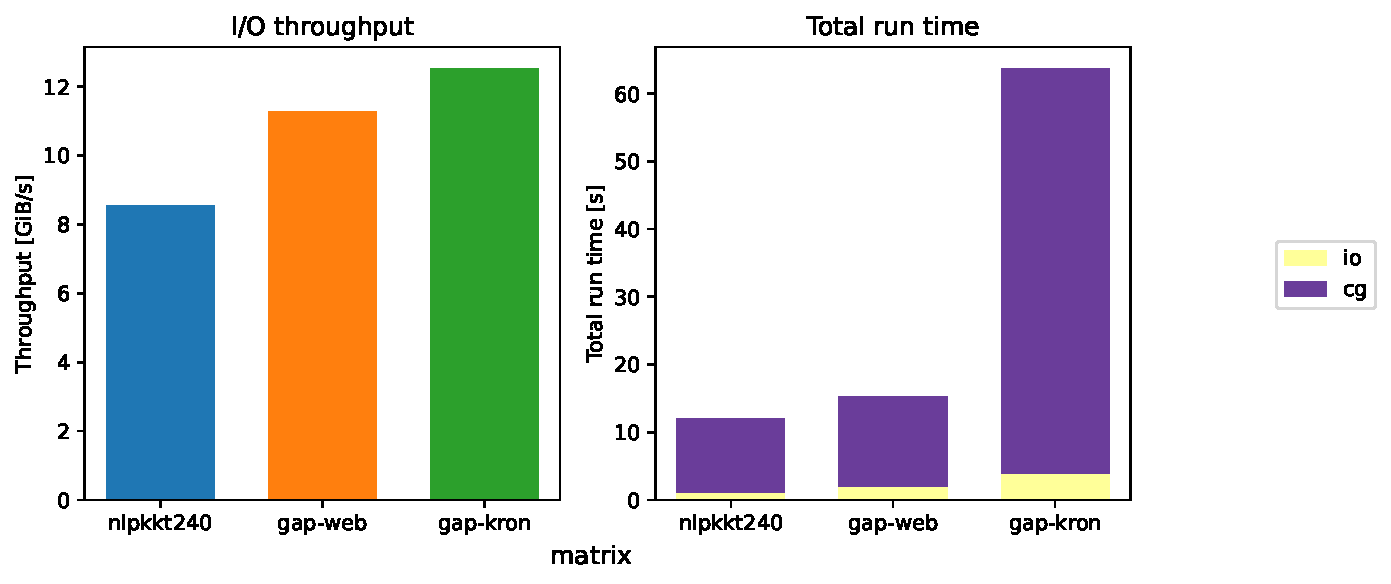
\includegraphics[scale=0.58]{static/io_mp.pdf}
    \caption{Time spent doing IO vs CG (8-1-16 layout)}
\end{figure}

\section{PETSc}

To compare the distributed sparse matrix-vector multiplication (D-CSR5) implemented by \csre{dim}
to a state of the art BLAS library, an
implementation of conjugate gradient solver using \csre{PETSc} (v3.15.1) introduced in
Section~\ref{tech:petsc} was created.

\csre{PETSc} supports
multiple storage formats for sparse matrices such as compressed sparse row, block compressed
sparse row, etc. The default for distributed sparse matrices, which is compressed sparse row
(PETSc \csre{MatType} \csre{MATMPIAIJ}~\cite{petsc-user-ref}) was used for benchmarking.

Furthermore, since \csre{PETSc} is a general-purpose library, some tradeoffs had to be made
in the benchmarking code. Even though \csre{PETSc} has its own conjugate gradient implementation
(\csre{KSPCG}),
the goal of the benchmark is to compare the performance of distributed sparse matrix-vector
multiplication, not the conjugate gradient implementation as a whole. To improve the granularity
of benchmarked sections, an alternative
implementation was produced to enable the timing of separate steps of the iteration instead of just
timing the whole iteration step.

As the benchmark is using CSR as a storage format,
each process of \csre{PETSc} solver loads a sub-section of the input matrix' rows of the same size (except possibly the last
process. Non-zero elements in the matrices used for benchmarking are distributed fairly
evenly across these sections\footnote{Heatmaps can be generated by running  \csre{dim_cli generate_heatmap <input_matrix>}.},
so this approach yields good load distribution across all processes.

\begin{figure}[htp]
    \centering
    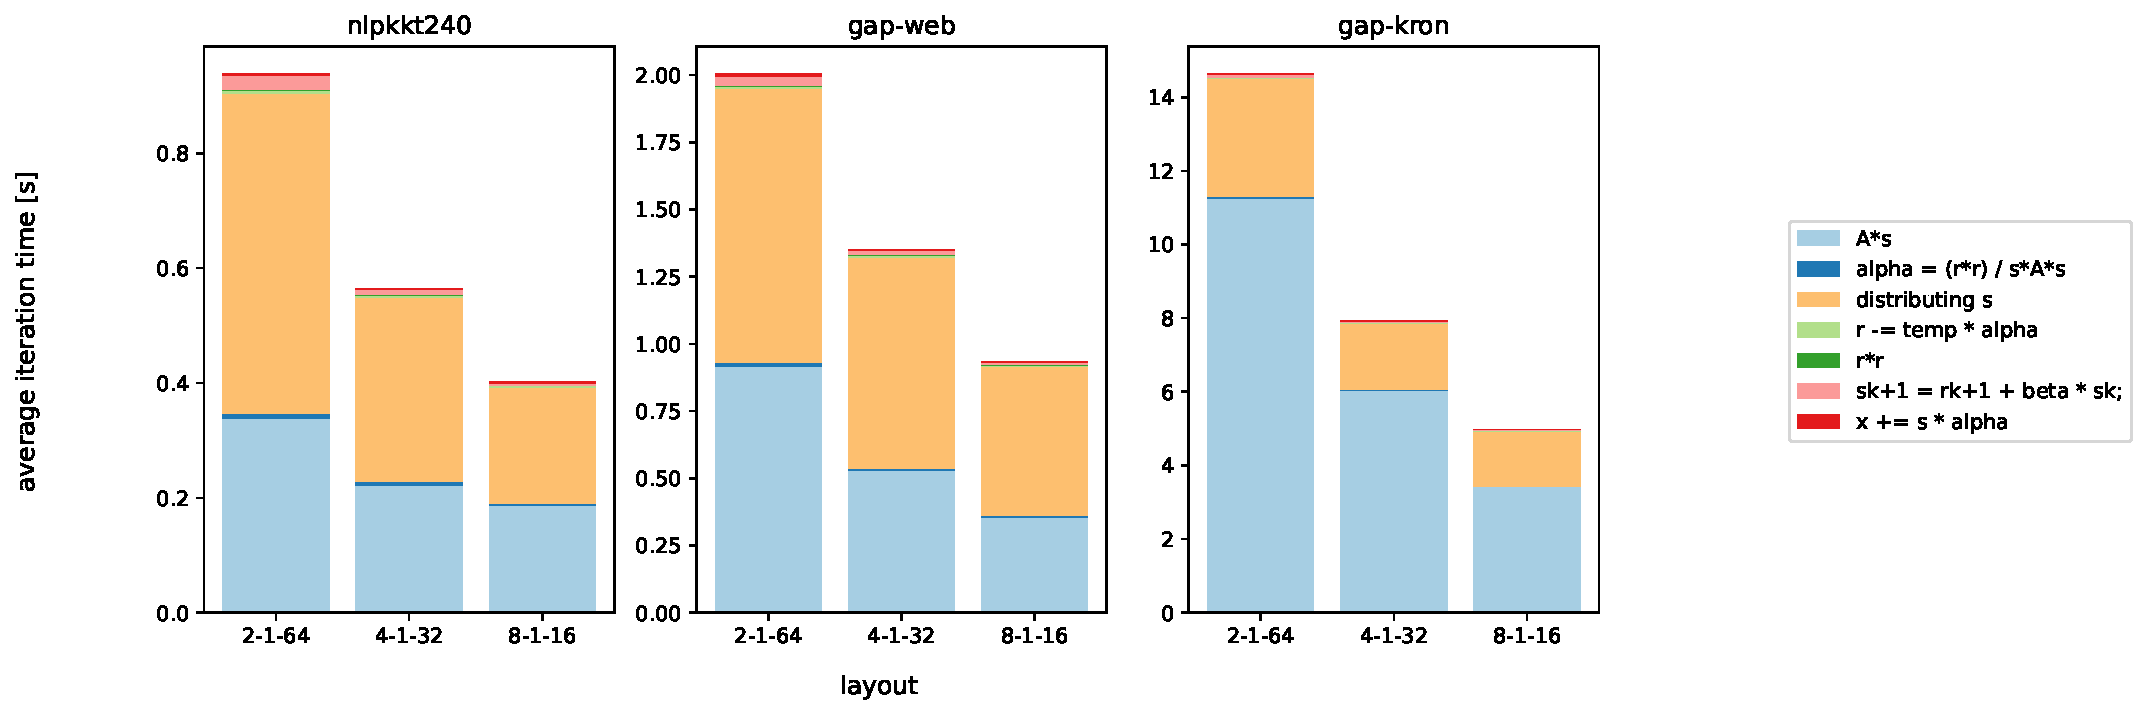
\includegraphics[scale=0.5]{static/petsc_mpi.pdf}
    \caption{PETSc implementation benchmark results}
\end{figure}

The benchmark results show that a significant portion of time each iteration is spent in the \texttt{distributing s}
step. This issue partly stems from a design decision made in PETSc. The distributed vectors (such as \csre{s})
have local size (size of vector part physically present in process) and global size (size of the whole vector).
For vector-vector operations such as \csre{axpy} or dot product, PETSc requires the participating vectors to
have the same local size. Since each process may require any element from
\csre{s}\footnote{Because any element in a row of sparse matrix can be non-zero.} it must have whole \csre{s}
in its memory. To obtain a sub-vector of \csre{s}, suitable for distributed \csre{sAs} a process must call
\csre{VecGetSubVector} and then restore said sub-vector in \csre{s} by calling \csre{VecRestoreSubVector}.

However, \csre{VecGetSubVector} may allocate new memory to store the sub-vector in, releasing said memory
when \csre{VecRestoreSubVector} is called, thus skewing the actual time needed for synchronization of
\csre{s} itself. For this reason, the \texttt{distributing s} step will not be considered when comparing
the two implemen\-tations.

\begin{figure}[htp]
    \centering
    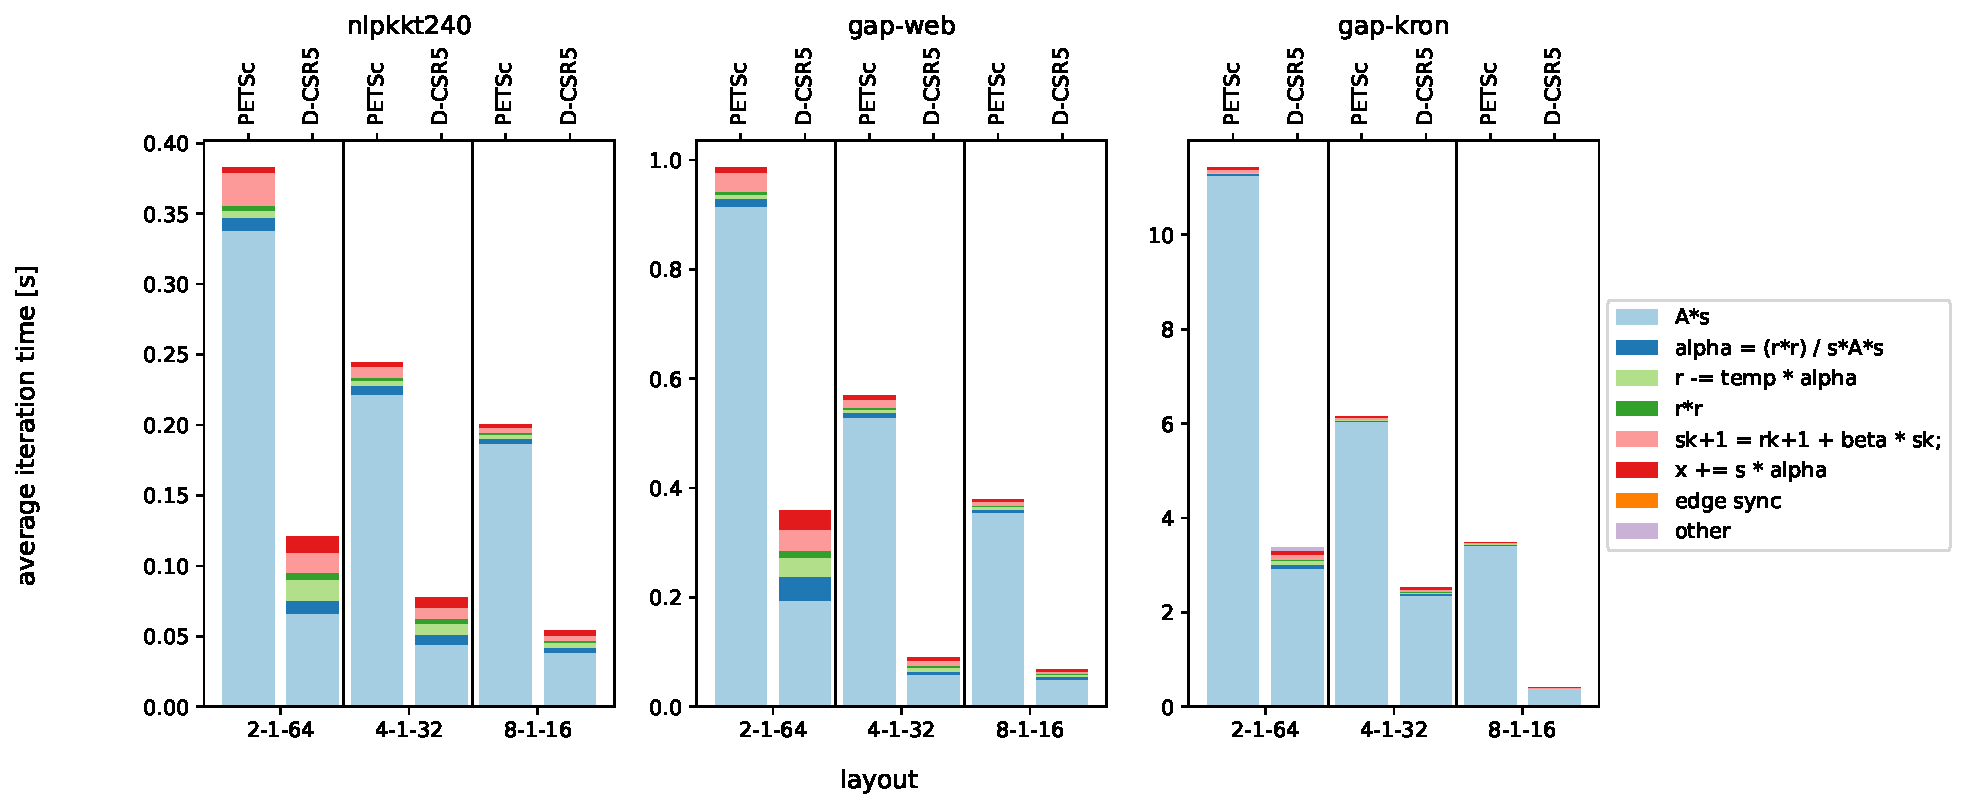
\includegraphics[scale=0.5]{static/petsc_vs_dim.pdf}
    \caption{PETSc vs D-CSR5 benchmark results (no synchronization)}\label{bench:petsc:vsDim}
\end{figure}

Even with the \texttt{distributing s} step removed, benchmark results (visualized in
Figure~\ref{bench:petsc:vsDim}) show that D-CSR5 implementation performs better
on all the benchmarked configurations. The speedup of D-CSR5 based implementation compared to \csre{PETSc}
ranges from 2.4 and 2.57x for iteration and SpMV steps respectively up to 8.5 and 9.46x. Speedup over every
layout and input matrix combination is shown in Figure~\ref{bench:petsc:table}.


\begin{figure}[htp]
    \centering
    \begin{tabular}{*{7}{c}}
        \toprule
                        & \multicolumn{2}{c}{\textbf{nlpkkt240}} & \multicolumn{2}{c}{\textbf{gap-web}} & \multicolumn{2}{c}{\textbf{gap-kron}}                           \\
        \cmidrule(lr){2-3} \cmidrule(lr){4-5} \cmidrule(lr){6-7}
        \textbf{layout} & iteration                              & As                                   & iteration                             & As   & iteration & As   \\
        \midrule
        \csre{2-1-64}   & 3.72                                   & 4.81                                 & 2.75                                  & 4.69 & 3.4       & 3.83 \\
        \csre{4-1-32}   & 3.14                                   & 5.04                                 & 6.27                                  & 9.04 & 2.43      & 2.57 \\
        \csre{8-1-16}   & 3.72                                   & 4.81                                 & 5.57                                  & 7.03 & 8.53      & 9.46 \\
        \bottomrule
    \end{tabular}
    \caption{Speedup of iteration and SpMV step of iteration using when using D-CSR5 vs PETSc}\label{bench:petsc:table}
\end{figure}


\setsecnumdepth{part}
\chapter{Conclusion}

This thesis aimed to research and evaluate the viability of distributing sparse matrix-vector multiplication
among multiple computational nodes using MPI\@. To that end, coordinate (COO) and compressed sparse row (CSR) formats
were reviewed, as well as Compressed Sparse Row 5 format introduced in~\cite{liu2015csr5}.

On-disk storage formats for sparse matrices were reviewed. Namely Matrix Market Exchange Format
and HDF5 backed format used by MATLAB v7.3. After reviewing existing formats, a storage scheme for CSR5 was 
devised
using HDF5 as underlying format, nullifying the need for conversion from CSR to CSR5 each time a matrix
is loaded.

The parallel SpMV algorithm outlined in~\cite{liu2015csr5} was implemented using C++20. Routines for
loading and storing sparse matrices as well as converting between sparse matrix formats were
also implemented. These were packaged into a library/toolkit named \csre{dim}.

The building blocks from \csre{dim} were then used to build distributed SpMV\@. Using MPI, SpMV was
distributed among multiple processes, with the CSR5 SpMV re-implementation used to perform partial
multiplication inside each process. Leveraging the MPI-IO capabilities of HDF5 library~\cite{hdf5} to load only
relevant parts of the matrix to minimize the time spent performing I/O operations. An algorithm for
synchronizing and distributing the partial results was then outlined and implemented.

This distributed solution was then benchmarked, using conjugate gradient method implementation, against the
single-process solution. These benchmarks clearly show that distributing the sparse matrix-vector multiplication
for large sparse matrices can lead to significant speed-up even though the result needs to be synchronized
and distributed amongst all processes each iteration.

To compare the performance of this solution against a battle-tested implemen\-tation conjugate gradient method
was also implemented using \texttt{PETSc} toolkit and then benchmarked. Comparing the average per-iteration times
suggests that the approach implemented in \csre{dim} leads to non-negligible speed ups.

Future directions include researching algorithms other than conjugate gradient in which SpMV is the
most computationally intensive task and the viability of distributing it. The on-disk storage format
introduced by this thesis may also benefit from more generalization, as it is currently quite specific to
CPU-only implementation of SpMV and thus not suitable for GPU or CPU/GPU heterogeneous implementations.


\bibliographystyle{iso690}
\bibliography{ref}

\setsecnumdepth{all}
\appendix


\chapter{Conjugate gradient method}\label{app:cg}

The conjugate gradient algorithm (abbr. CG) is one of the best known iterative methods which can be used to solve large
symmetric positive definite linear systems~\cite{saad03:IMS}. The algorithm in its iterative form is outlined
in Alogithm~\ref{app:cg:algo}.

\begin{algorithm}
    \caption{Iterative conjugate gradient}\label{app:cg:algo}
    \begin{algorithmic}
        \Function{conjugate\_gradient}{$\var{A}$, $\var{b}$, $\var{x}$}
        \State $\var{r} \gets \var{b - Ax}$
        \State $\var{s} \gets \var{r}$
        \State $\var{r\_r} \gets \var{r} \cdot \var{r}$

        \For{$\var{i} = 0; \var{i} < \var{max\_iters}; \var{++i}$}
        \State $\var{As} \gets \var{A} \cdot \var{s}$
        \State $\var{alpha} \gets \frac{\var{r\_r}}{\var{s'} \cdot \var{As}} $
        \State $\var{x} \gets \var{x} + \var{alpha} \cdot \var{s}$
        \State $\var{r} \gets \var{r} - \var{alpha} \cdot \var{As}$
        \State $\var{r\_r\_new} \gets \var{r'} \cdot \var{r}$

        \If{$\var{sqrt(r\_r\_new)} < \var{threshold}$}
        \State $\textbf{break}$
        \EndIf

        \State $\var{beta} \gets \frac{\var{r\_r\_new}}{\var{r\_r}}$
        \State $\var{r\_r} \gets \var{r\_r\_new}$
        \State $\var{s} \gets \var{r} + \var{beta} \cdot \var{s}$

        \EndFor

        \EndFunction
    \end{algorithmic}
\end{algorithm}

\section{Distributed conjugate gradient implementation}\label{dcg:steps}

Each process first obtains a full copy of \csre{s}.
Then the steps of the algorithm above are performed as follows with each step being labeled as 
\texttt{CG<num>} for the steps of the actual algorithm and \texttt{DCG<num>} for the steps 
only the distributed version performs.

\textbf{Step \texttt{CG0}}: $\var{As} \gets \var{A} \cdot \var{s}$. Each process can perform SpMV on its local part of
\csre{A}. This SpMV will result, in each process having part of \csre{As}, with some overlapping
output elements having only part of its value which needs to be synchronized.

\textbf{Step \texttt{DCG0.1}}: edge sync. After SpMV is done, the synchronization for overlapping 
edge elements described in Section~\ref{dspmv:sync} can begin.

\textbf{Step \texttt{CG1}}: $\var{alpha} \gets \frac{\var{r\_r}}{\var{s} \cdot \var{As}}$. Since each process only has part of
\csre{As} and full \csre{s}, it can do its part of the $\var{s} \cdot \var{As}$.
Dot product of two vectors is computed as $x \cdot y = \sum x_i \cdot y_i$, so $\var{s} \cdot \var{As}$
can be rewritten as $a \cdot As = \sum_{p=0}^{np} \sum_{i=os_p}^{oe_p} s_i \cdot As_{i-os_p}$ where
$np$ is number of processes, and $os_p$ and $oe_p$ denote start and end of output for process
$p$ respectively.The outer sum can be computed using \csre{MPI_Allreduce},
summing the results of inner sum for each process.

For the elements that need to be synchronized (multiple processes are computing their sub-values),
the resulting element is a sum of all of the sub-results thus $s \cdot As = \sum s_i \cdot As_i$ term for $i$
which is computed by multiple processes can be rewritten as $s_i \cdot (As_{i_{p1}} + ... + As_{i_{pn}})$.
As multiplication in $R$ is distributive, this can be rewritten as $s_i \cdot As_{i_{p1}} + ... + s_i \cdot As_{i_{pn}}$
so there is no need to synchronize $As_i$ as result will be synchronized when partial results for
each process are summed.

\textbf{Step \texttt{CG2}}: $\var{x} \gets \var{x} + \var{alpha} \cdot \var{s}$ each process only has the part of \csre{x},
coinciding with the output ranges into \csre{As} it owns. Thus thus each process only
modifies said part of \csre{x}.

\textbf{Step \texttt{CG3}}: $\var{r} \gets \var{r} - \var{alpha} \cdot \var{As}$ Similarly to previous step, each process
only modifies the part of residual vector \csre{r}. Synchronization of overlapping
output elements for \csre{As} must be done before this step, as process which owns the
element uses it to modify \var{r} in this step.

\textbf{Step \texttt{CG4}}: $\var{r\_r\_new} \gets \var{r'} \cdot \var{r}$ Same as in alpha computation, the dot product
can be divided into sub sums, which can then be summed across all processes, using
\csre{MPI_Allreduce}.

\textbf{Step \texttt{DCG0.1}}: edge sync. The second part of \texttt{DCG0}, which calls \csre{MPI_Waitall}
to wait until the sync is over as the owning processes need to have the correct values in \csre{s}.

\textbf{Step \texttt{CG5}}: $\var{s} \gets \var{r} + \var{beta} \cdot \var{s}$ each process computes only part of new
\csre{s}, corresponding to its output range in \csre{As}. 

\textbf{Step \texttt{DCG0.1}}: distributing \csre{s}. The resulting \csre{s} is
then distributed to all processes using same algorithm as described in section
about synchronization of distributed SpMV results using \csre{MPI_Allgatherv}.
This distribution step is the heaviest as far as MPI communication goes.

Note that this algorithm may be further optimized as described in~\cite{distCGwRedSync}, but
since it is only used as a test-bed for benchmarking implementation in \csre{dim} these are not
implemented.

\chapter{Building dim}

This chapter describes the process of obtaining dependencies, configuring, and building \texttt{dim} as well
as optional benchmarks.

\section{Dependencies}\label{bdim:deps}

\csre{dim} uses \csre{cmake} as its meta build-system. Only recent versions of CMake (3.20-3.22) were tested.

The code uses C++20 features and as such, needs a C++20 capable compiler. Tested compilers
are:

\begin{itemize}
    \item GCC 10.3.0 (available on RCI)
    \item GCC 11.1.0
    \item Clang 12.1.0 (available on RCI)
    \item Clang 13.0.1
\end{itemize}
\csre{dim} is also built by GitHub Actions CI by clang 13 as well as linted by clang-tidy on each commit.

\csre{conan} is used for package management. \csre{conan} is implemented in Python and can be
obtained from \csre{pip}. The project will invoke \csre{conan} automatically when \csre{cmake} configure step
is running, so it should be transparent to the user. If the code is built locally (meaning not on RCI cluster),
some packages hosted on a private Artifactory instance of the author are needed. The following commands
have to be executed to add the remote:

\begin{minted}[]{bash}
    # the remote requires revisions to 
    # be enabled in local conan installation
    conan config set general.revisions_enabled=1
    # this hosts the PETSc package recipe as well
    # as some prebuilt libraries.
    conan remote add rurabori-conan \
        https://rurabori.jfrog.io/artifactory/api/conan/rurabori-conan
    cmake . -B build # cmake arguments as usual ...
\end{minted}

When building on the RCI cluster, it may be beneficial
to use the provided libraries optimized for the nodes they will be running on. To enable this,
pass \mintinline{bash}{-Dsystem_scientific_libs="ON"} to \csre{cmake} when configuring. There is a script
at \csre{scripts/rci/slurm_cmake} which will automatically load modules needed for compilation and offload
the configuration/compilation step to a computational node.

\section{Building the binaries}

The project provides only two configuration options immediately relevant to this thesis. The
first one is \csre{enable_petsc_benchmark} which is disabled by default. If it is enabled,
the PETSc implementation of the distributed conjugate gradient will be built, and the project
will require PETSc as a dependency. The second option is \csre{system_scientific_libs} which
was explained in~\ref{bdim:deps}. Both of these options can be enabled/disabled by passing
\csre{-D<option>="ON/OFF"} to \csre{cmake} during configuration phase.

A typical RCI configuration might look like this:
\begin{minted}[]{bash}
    cd <project_directory>
    cmake . -B build \
            -Dsystem_scientific_libs="ON" \
            -Denable_petsc_benchmark="ON" \
            -DENABLE_TESTING="OFF" \
            -G "Unix Makefiles" \
            -DCMAKE_BUILD_TYPE=Release
    cmake --build build
\end{minted}

The resulting binaries will be in the build directory, in subfolders matching the structure of
the repository i.e. \csre{dim_cli} which is defined in folder \csre{apps/dim_cli} will be found
in \csre{build/apps/dim_cli} folder. Alternatively the project can be installed as a SLURM module
after it is built by running:

\begin{minted}[]{bash}
    cmake --install build \
          --prefix <install_dir>/dim
    MODULEPATH="$MODULEPATH:<install_dir>"
    # from here on, dim should behave as any other module
    ml dim
    dim_cli --version
\end{minted}

\section{Available executables}

\csre{dim} build produces multiple executables. Benchmarks which were used to produce data for this thesis as
well as \csre{dim_cli}, a command-line utility with multiple subcommands for downloading/converting and
working with sparse matrices in general. Only the CLI will be explained as the benchmarks map well to
graphs in this thesis, so they should be pretty self-explanatory.

\subsection{dim\_cli}

\csre{dim_cli} is a command-line utility which provides four subcommands
\footnote{dim\_cli supports \csre{-h/--help} for the top-level executable as well as for each subcommand for more detailed argument listing.}:
\begin{itemize}
    \item \csre{store_matrix}
    \item \csre{compare_results}
    \item \csre{download}
    \item \csre{generate_heatmap}
\end{itemize}

\csre{store_matrix} subcommand takes a path to matrix in MMEF or Matlab compatible HDF5 format, and stores
the matrix in CSR or CSR5 format (provided to the \csre{-f} flag) into a HDF5 file. The command also
requires a configuration file, which describes properties for the HDF5 groups in which the data will be
stored. A sample config is stored in \csre{resources/config.yaml} and installed into \csre{share} directory
when \csre{dim} is installed as a SLURM module.

\begin{minted}{bash}
    # convert MMEF to CSR5.
    dim_cli store_matrix matrix.mtx \
                         -f csr5 \
                         -c resources/config.yaml
    # will produce matrix.csr5.h5
\end{minted}

\csre{compare_results} takes a path to HDF5 file (or two files), with result vectors and compares them.
This command is mainly useful for checking the results are correct and stable across implementations.

\begin{minted}{bash}
    # compare two result vectors.
    dim_cli compare_results res.h5 -l "/Y1" -r "/Y2"
\end{minted}

\csre{download} subcommand retrieves a matrix from an URL provided as an argument and unpacks it while
downloading, saving some time as the used matrices are fairly large.

\begin{minted}{bash}
    # downlaod and unpack matrix from <URL> into 
    # resources/matrices directory.
    dim_cli download <URL> -d resources/matrices
\end{minted}

\csre{generate_heatmap} expects a path to matrix in CSR5 format introduced in Section~\ref{csr5:onDisk}.
It will produce a black and white PNG image, with the brightness reflecting the number of non-zero elements
of the segment of the matrix the pixel represents.

\begin{minted}{bash}
    dim_cli generate_heatmap mat.csr5.h5
    # mat.png will be produced
\end{minted}

\begin{figure}[htp]
    \begin{minipage}{0.5\textwidth}
        
\includegraphics[trim=0 2500 2500 0, clip, scale=0.1]{static/e40r5000.png}
    \end{minipage}
    \begin{minipage}{0.5\textwidth}
        
\includegraphics[trim=0 2500 2500 0, clip, scale=0.1]{static/e40r5000.dist.png}
    \end{minipage}
    \caption{Zoomed-in example of a generated heat/distribution maps.}
\end{figure}

However, this command will behave a bit differently when process count \csre{-p} is specified. It will not
reflect the density structure as precisely as the black and white output, coloring the pixels
with a different color for each process instead. Resolution can also be specified by providing 
\csre{-r <width> <height>} if a finer structure needs to be captured (or the matrix is large).



\chapter{Acronyms}
% \printglossaries
\begin{description}
    \item[COO] Coordinate Format
    \item[CSR] Compressed Sparse Row Format
    \item[CSR5] Compressed Sparse Row 5 Format
    \item[CLI] Command Line Interface
    \item[$n_{nz}$] Number of non-zero elements in a sparse matrix
    \item[HDF5] Hierarchical Data Format v5
    \item[dim]  The library implemented during result for this thesis
    \item[PETSc] Portable, Extensible Toolkit for Scientific computation
    \item[CG] conjugate gradient method
    \item[SpMV] Sparse Matrix-Vector multiplication
    \item[SSE] Streaming SIMD Extensions
    \item[AVX] Advanced Vector Extensions
\end{description}


\chapter{Contents of enclosed CD}

%change appropriately
\dirtree{%
    .1 readme.txt\DTcomment{the file with CD contents description}.
    .1 exe\DTcomment{the directory with executables}.
    .1 src\DTcomment{the directory of source codes}.
    .2 wbdcm\DTcomment{implementation sources}.
    .2 thesis\DTcomment{the directory of \LaTeX{} source codes of the thesis}.
    .1 thesis.pdf\DTcomment{the thesis text in PDF format}.
}

\end{document}
